
\documentclass[11pt,a4paper]{article}
\usepackage{fontspec}
\usepackage{polyglossia}
\setmainlanguage{spanish}
\setmainfont{TeX Gyre Pagella}
\setmonofont{DejaVu Sans Mono}[Scale=0.8]
\emergencystretch=3em
\usepackage[margin=2.5cm]{geometry}
\usepackage{booktabs,longtable,array,graphicx,xcolor,colortbl,listings,fancyhdr,titlesec,enumitem,caption,float,pdflscape,microtype,amssymb,amsmath}
\usepackage[hidelinks]{hyperref}
\definecolor{azul}{HTML}{1F3A5F}
\definecolor{celda}{HTML}{E4EEF9}
\definecolor{gris}{HTML}{F5F5F5}
\definecolor{verde}{HTML}{2E7D32}
\titleformat{\section}{\Large\bfseries\color{azul}}{\thesection}{0.6em}{}
\titleformat{\subsection}{\large\bfseries\color{azul}}{\thesubsection}{0.6em}{}
\titleformat{\subsubsection}{\normalsize\bfseries\color{azul}}{\thesubsubsection}{0.6em}{}
\setlength{\parskip}{4pt}
\pagestyle{fancy}\fancyhf{}
\fancyhead[L]{\small INFO1148 --- Proyecto de Análisis Sintáctico}
\fancyhead[R]{\small DomoDSL}
\fancyfoot[C]{\thepage}
\renewcommand{\headrulewidth}{0.3pt}
\captionsetup{font=small,labelfont=bf}
\lstset{basicstyle=\ttfamily\footnotesize, numbers=left, numberstyle=\tiny\color{gray}, numbersep=6pt,
  breaklines=true, breakatwhitespace=false, frame=single, rulecolor=\color{gray!60}, backgroundcolor=\color{gris},
  language=Python, keywordstyle=\color{azul}\bfseries, commentstyle=\color{verde}\itshape,
  stringstyle=\color{red!50!black}, showstringspaces=false, tabsize=4, columns=fullflexible,
  captionpos=b, xleftmargin=1.2em, framexleftmargin=1.2em}
\newcommand{\ok}{\textcolor{verde}{\ensuremath{\checkmark}}}
\begin{document}

\begin{titlepage}
\centering
{\large Universidad Católica de Temuco\\ Ingeniería Civil Informática\par}
\vspace{0.6cm}
{\large Teoría de la Computación --- INFO1148\par}
\vspace{2.2cm}
{\Large\bfseries\color{azul} Proyecto: Diseño e implementación de un analizador sintáctico\par}
\vspace{0.6cm}
{\Huge\bfseries\color{azul} DomoDSL\par}
\vspace{0.3cm}
{\large Un lenguaje de reglas para la automatización de una casa inteligente (IoT)\par}
\vspace{1.4cm}
{\large Gramática libre de contexto \textperiodcentered{} FIRST y FOLLOW \textperiodcentered{} Tabla LL(1)\\
Parser predictivo \textperiodcentered{} AST \textperiodcentered{} Manejo de errores\par}
\vspace{2.6cm}
\begin{tabular}{rl}
\textbf{Integrantes:} & [Nombre Apellido 1] \\
 & [Nombre Apellido 2] \\
 & [Nombre Apellido 3] \\[6pt]
\textbf{Docente:} & [Nombre del docente] \\[6pt]
\textbf{Fecha:} & Octubre de 2026 \\[6pt]
\textbf{Repositorio:} & \texttt{https://github.com/[usuario]/[repositorio]}
\end{tabular}
\vfill
{\small Implementación en Python 3 \textperiodcentered{} sin generadores de parsers \textperiodcentered{} solo biblioteca estándar\par}
\end{titlepage}
\tableofcontents
\clearpage
\newcommand{\parte}{1}
% Secciones 1, 10, 11, 12 y anexos (tarea R3) - autor: Persona C.
% \parte=1 imprime la introduccion; \parte=2 imprime pruebas, conclusiones y anexos.
\ifnum\parte=1

\section{Introducción y dominio seleccionado}

Los lenguajes de programación y los lenguajes de dominio específico (DSL) necesitan mecanismos que verifiquen si
una secuencia de símbolos cumple una estructura formal. Este proyecto diseña e implementa, \emph{desde cero},
un analizador sintáctico para un pequeño DSL, aplicando los contenidos del curso: gramáticas libres de contexto (GLC),
eliminación de recursión por la izquierda, factorización, conjuntos FIRST y FOLLOW, tabla predictiva LL(1),
construcción de árboles sintácticos y detección de errores.

\paragraph{Dominio escogido.} Se eligió la \textbf{automatización de una casa inteligente (IoT)}, el ejemplo
orientativo del enunciado. El usuario describe \emph{reglas} del tipo ``cuando ocurra esta condición, ejecuta estas acciones'':
\begin{center}\texttt{WHEN temperatura > 28 AND humedad < 40 THEN encender ventilador;}\end{center}
Este dominio es adecuado porque (i)~las reglas condición--acción son naturales y fáciles de validar, (ii)~las condiciones admiten
conectores lógicos, negación y agrupación, lo que obliga a resolver precedencia y asociatividad en la gramática, y
(iii)~las acciones admiten parámetros, lo que enriquece la sintaxis sin perder la propiedad LL(1).

\paragraph{Alcance.} El lenguaje se llama \textbf{DomoDSL}. Se entregan: la especificación del lenguaje, la GLC y su
análisis, FIRST/FOLLOW, la tabla LL(1), \textbf{dos} analizadores predictivos (descenso recursivo y dirigido por tabla),
AST y árbol de derivación, mensajes de error localizados, 46 casos de prueba y 18 pruebas unitarias.

\paragraph{Estructura del informe.} Sigue la organización sugerida en el enunciado: especificación del lenguaje
(sección~2), gramática (3), análisis (4), FIRST y FOLLOW (5), tabla LL(1) (6), parser (7), árboles (8), errores (9),
pruebas (10), conclusiones (11) y anexos (12).

\fi
\ifnum\parte=2

\section{Casos de prueba}

Se documentan \textbf{46 casos}: 12 válidas, 20 inválidas y 14 casos límite (el enunciado exige 10, 10 y 5; la rúbrica premia
25 o más pruebas variadas). Cada caso se ejecutó con \textbf{ambos analizadores}; el resultado de las tablas es el obtenido por el programa
(\texttt{python ejecutar\_pruebas.py}). Resultado global: \textbf{46/46 casos correctos}.
Además hay 18 pruebas unitarias (\texttt{python -m unittest}) que verifican el léxico, FIRST, FOLLOW, la ausencia de conflictos, la precedencia
y asociatividad del AST y la posición de los errores. Los casos de entradas muy largas (L05--L07) se muestran abreviados; su texto completo se genera
en \texttt{casos\_prueba.py}.

\begin{landscape}
\subsection{Entradas sintácticamente válidas}
\begin{longtable}{@{}>{\raggedright\arraybackslash}p{0.9cm} >{\raggedright\arraybackslash}p{6.4cm} >{\raggedright\arraybackslash}p{3.2cm} >{\raggedright\arraybackslash}p{6.8cm} >{\raggedright\arraybackslash}p{4.4cm}@{}}
\toprule
\textbf{ID} & \textbf{Entrada} & \textbf{Resultado esperado} & \textbf{Resultado obtenido} & \textbf{Observación} \\
\midrule
\endhead
V01 & \footnotesize \texttt{WHEN temperatura > 28 THEN encender ventilador;} & \footnotesize ACEPTA & \footnotesize ACEPTA \ok & \footnotesize Regla mínima del enunciado \\
\addlinespace[2pt]
V02 & \footnotesize \texttt{WHEN movimiento == TRUE THEN activar alarma;} & \footnotesize ACEPTA & \footnotesize ACEPTA \ok & \footnotesize Valor booleano \\
\addlinespace[2pt]
V03 & \footnotesize \texttt{WHEN temperatura > 28 AND humedad < 40 THEN encender ventilador;} & \footnotesize ACEPTA & \footnotesize ACEPTA \ok & \footnotesize Conector AND \\
\addlinespace[2pt]
V04 & \footnotesize \texttt{WHEN luz < 100 OR hora >= 20 THEN encender lampara;} & \footnotesize ACEPTA & \footnotesize ACEPTA \ok & \footnotesize Conector OR y operador >= \\
\addlinespace[2pt]
V05 & \footnotesize \texttt{WHEN NOT puerta == TRUE THEN activar alarma;} & \footnotesize ACEPTA & \footnotesize ACEPTA \ok & \footnotesize Extensión: NOT \\
\addlinespace[2pt]
V06 & \footnotesize \texttt{WHEN (temperatura > 30 OR humedad > 80) AND presencia == TRUE THEN encender aire;} & \footnotesize ACEPTA & \footnotesize ACEPTA \ok & \footnotesize Extensión: paréntesis (agrupación) \\
\addlinespace[2pt]
V07 & \footnotesize \texttt{WHEN temperatura > 28 THEN encender ventilador 3, activar alarma;} & \footnotesize ACEPTA & \footnotesize ACEPTA \ok & \footnotesize Extensión: múltiples acciones y parámetro \\
\addlinespace[2pt]
V08 & \footnotesize \texttt{WHEN temperatura >= 26.5 THEN ajustar termostato 22 TRUE;} & \footnotesize ACEPTA & \footnotesize ACEPTA \ok & \footnotesize Número decimal y varios parámetros \\
\addlinespace[2pt]
V09 & \footnotesize \texttt{WHEN temperatura > 28 THEN encender ventilador;\textbackslash{}nWHEN movimiento == TRUE THEN activar alarma;} & \footnotesize ACEPTA & \footnotesize ACEPTA \ok & \footnotesize Dos reglas en líneas distintas \\
\addlinespace[2pt]
V10 & \footnotesize \texttt{WHEN a != b THEN x y;} & \footnotesize ACEPTA & \footnotesize ACEPTA \ok & \footnotesize Comparación ID contra ID \\
\addlinespace[2pt]
V11 & \footnotesize \texttt{WHEN NOT NOT a == 1 THEN x y;} & \footnotesize ACEPTA & \footnotesize ACEPTA \ok & \footnotesize NOT anidado \\
\addlinespace[2pt]
V12 & \footnotesize \texttt{WHEN a > 1 AND (b < 2 OR NOT (c == TRUE)) THEN x y 1 2 3 TRUE FALSE z;} & \footnotesize ACEPTA & \footnotesize ACEPTA \ok & \footnotesize Combina NOT, paréntesis y lista larga de parámetros \\
\addlinespace[2pt]
\bottomrule
\end{longtable}
\subsection{Entradas sintácticamente inválidas}
\begin{longtable}{@{}>{\raggedright\arraybackslash}p{0.9cm} >{\raggedright\arraybackslash}p{6.4cm} >{\raggedright\arraybackslash}p{3.2cm} >{\raggedright\arraybackslash}p{6.8cm} >{\raggedright\arraybackslash}p{4.4cm}@{}}
\toprule
\textbf{ID} & \textbf{Entrada} & \textbf{Resultado esperado} & \textbf{Resultado obtenido} & \textbf{Observación} \\
\midrule
\endhead
I01 & \footnotesize \texttt{WHEN temperatura > 28 encender ventilador;} & \footnotesize RECHAZA (el mensaje menciona «la palabra reservada THEN») & \footnotesize RECHAZA \ok\newline \scriptsize Error sintáctico [1:23]: se esperaba la palabra reservada THEN (o un conector AND / OR) después de la condición, pero se encontró el identificador 'encender'. & \footnotesize Falta THEN \\
\addlinespace[2pt]
I02 & \footnotesize \texttt{WHEN temperatura > THEN encender ventilador;} & \footnotesize RECHAZA (el mensaje menciona «después del operador >») & \footnotesize RECHAZA \ok\newline \scriptsize Error sintáctico [1:20]: se esperaba un valor (número, TRUE, FALSE o identificador) después del operador >, pero se encontró la palabra reservada THEN. & \footnotesize Falta el valor tras el operador \\
\addlinespace[2pt]
I03 & \footnotesize \texttt{WHEN temperatura 28 THEN encender ventilador;} & \footnotesize RECHAZA (el mensaje menciona «después de 'temperatura'») & \footnotesize RECHAZA \ok\newline \scriptsize Error sintáctico [1:18]: se esperaba un operador relacional ('>', '<', '>=', '<=', '==', '!=') después de 'temperatura', pero se encontró el número 28. & \footnotesize Falta el operador relacional \\
\addlinespace[2pt]
I04 & \footnotesize \texttt{temperatura > 28 THEN encender ventilador;} & \footnotesize RECHAZA (el mensaje menciona «la palabra reservada WHEN») & \footnotesize RECHAZA \ok\newline \scriptsize Error sintáctico [1:1]: se esperaba la palabra reservada WHEN al inicio de una regla, pero se encontró el identificador 'temperatura'. & \footnotesize La regla no comienza con WHEN \\
\addlinespace[2pt]
I05 & \footnotesize \texttt{WHEN temperatura > 28 THEN encender ventilador} & \footnotesize RECHAZA (el mensaje menciona «';'») & \footnotesize RECHAZA \ok\newline \scriptsize Error sintáctico [1:47]: se esperaba ';' al final de la regla (o ',' para encadenar otra acción), pero se encontró el fin de la entrada. & \footnotesize Falta el punto y coma final \\
\addlinespace[2pt]
I06 & \footnotesize \texttt{WHEN temperatura > 28 THEN ;} & \footnotesize RECHAZA (el mensaje menciona «el nombre de una acción») & \footnotesize RECHAZA \ok\newline \scriptsize Error sintáctico [1:28]: se esperaba el nombre de una acción (identificador) después de THEN, pero se encontró el símbolo ';'. & \footnotesize Regla sin acción \\
\addlinespace[2pt]
I07 & \footnotesize \texttt{WHEN temperatura > 28 THEN encender;} & \footnotesize RECHAZA (el mensaje menciona «después de la acción 'encender'») & \footnotesize RECHAZA \ok\newline \scriptsize Error sintáctico [1:36]: se esperaba el dispositivo u objeto (identificador) después de la acción 'encender', pero se encontró el símbolo ';'. & \footnotesize Acción sin dispositivo \\
\addlinespace[2pt]
I08 & \footnotesize \texttt{WHEN (temperatura > 28 THEN encender ventilador;} & \footnotesize RECHAZA (el mensaje menciona «')' para cerrar el paréntesis») & \footnotesize RECHAZA \ok\newline \scriptsize Error sintáctico [1:24]: se esperaba ')' para cerrar el paréntesis abierto en la columna 6, pero se encontró la palabra reservada THEN. & \footnotesize Paréntesis sin cerrar \\
\addlinespace[2pt]
I09 & \footnotesize \texttt{WHEN temperatura > 28) THEN encender ventilador;} & \footnotesize RECHAZA (el mensaje menciona «sin su '(' correspondiente») & \footnotesize RECHAZA \ok\newline \scriptsize Error sintáctico [1:22]: paréntesis de cierre ')' sin su '(' correspondiente. & \footnotesize Paréntesis de cierre sobrante \\
\addlinespace[2pt]
I10 & \footnotesize \texttt{WHEN temperatura > 28 AND THEN encender ventilador;} & \footnotesize RECHAZA (el mensaje menciona «después de AND») & \footnotesize RECHAZA \ok\newline \scriptsize Error sintáctico [1:27]: se esperaba una condición (un identificador, NOT o '(') después de AND, pero se encontró la palabra reservada THEN. & \footnotesize AND sin segundo operando \\
\addlinespace[2pt]
I11 & \footnotesize \texttt{WHEN temperatura > 28 OR OR humedad < 3 THEN x y;} & \footnotesize RECHAZA (el mensaje menciona «después de OR») & \footnotesize RECHAZA \ok\newline \scriptsize Error sintáctico [1:26]: se esperaba una condición (un identificador, NOT o '(') después de OR, pero se encontró la palabra reservada OR. & \footnotesize Dos OR seguidos \\
\addlinespace[2pt]
I12 & \footnotesize \texttt{WHEN temperatura = 28 THEN encender ventilador;} & \footnotesize RECHAZA (el mensaje menciona «¿quiso escribir '=='») & \footnotesize RECHAZA \ok\newline \scriptsize Error léxico [1:18]: símbolo no reconocido '='. ¿quiso escribir '==' para comparar? & \footnotesize Error léxico: '=' en vez de '==' \\
\addlinespace[2pt]
I13 & \footnotesize \texttt{WHEN temperatura > 28 THEN encender ventilador;\textbackslash{}nWHEN humedad < 40 THEN encender bomba} & \footnotesize RECHAZA (el mensaje menciona «línea 2») & \footnotesize RECHAZA \ok\newline \scriptsize Error sintáctico [2:38]: se esperaba ';' al final de la regla (o ',' para encadenar otra acción), pero se encontró el fin de la entrada. & \footnotesize Segunda regla sin ';' (error localizado en la línea 2) \\
\addlinespace[2pt]
I14 & \footnotesize \texttt{WHEN 28 > temperatura THEN encender ventilador;} & \footnotesize RECHAZA (el mensaje menciona «el número 28») & \footnotesize RECHAZA \ok\newline \scriptsize Error sintáctico [1:6]: se esperaba una condición (un identificador, NOT o '(') después de WHEN, pero se encontró el número 28. & \footnotesize Un número a la izquierda del operador \\
\addlinespace[2pt]
I15 & \footnotesize \texttt{WHEN temperatura > 28 THEN encender ventilador @;} & \footnotesize RECHAZA (el mensaje menciona «símbolo no reconocido '@'») & \footnotesize RECHAZA \ok\newline \scriptsize Error léxico [1:48]: símbolo no reconocido '@'. & \footnotesize Error léxico: carácter no válido \\
\addlinespace[2pt]
I16 & \footnotesize \texttt{WHEN temperatura > 28 THEN encender ventilador;;} & \footnotesize RECHAZA (el mensaje menciona «una nueva regla (WHEN) o el fin de la entrada») & \footnotesize RECHAZA \ok\newline \scriptsize Error sintáctico [1:48]: se esperaba una nueva regla (WHEN) o el fin de la entrada después de ';', pero se encontró el símbolo ';'. & \footnotesize Punto y coma duplicado \\
\addlinespace[2pt]
I17 & \footnotesize \texttt{WHEN temperatura > 28 THEN encender ventilador, ;} & \footnotesize RECHAZA (el mensaje menciona «después de ','») & \footnotesize RECHAZA \ok\newline \scriptsize Error sintáctico [1:49]: se esperaba el nombre de una acción (identificador) después de ',', pero se encontró el símbolo ';'. & \footnotesize Coma sin acción posterior \\
\addlinespace[2pt]
I18 & \footnotesize \texttt{WHEN NOT THEN x y;} & \footnotesize RECHAZA (el mensaje menciona «después de NOT») & \footnotesize RECHAZA \ok\newline \scriptsize Error sintáctico [1:10]: se esperaba una condición (un identificador, NOT o '(') después de NOT, pero se encontró la palabra reservada THEN. & \footnotesize NOT sin operando \\
\addlinespace[2pt]
I19 & \footnotesize \texttt{WHEN a > 1 THEN x y WHEN b < 3 THEN z w;} & \footnotesize RECHAZA (el mensaje menciona «la palabra reservada WHEN») & \footnotesize RECHAZA \ok\newline \scriptsize Error sintáctico [1:21]: se esperaba ';' al final de la regla (o ',' para encadenar otra acción), pero se encontró la palabra reservada WHEN. & \footnotesize Falta ';' entre dos reglas \\
\addlinespace[2pt]
I20 & \footnotesize \texttt{WHEN a > 1 THEN 5 ventilador;} & \footnotesize RECHAZA (el mensaje menciona «el nombre de una acción») & \footnotesize RECHAZA \ok\newline \scriptsize Error sintáctico [1:17]: se esperaba el nombre de una acción (identificador) después de THEN, pero se encontró el número 5. & \footnotesize La acción debe ser un identificador \\
\addlinespace[2pt]
\bottomrule
\end{longtable}
\subsection{Casos límite}
\begin{longtable}{@{}>{\raggedright\arraybackslash}p{0.9cm} >{\raggedright\arraybackslash}p{6.4cm} >{\raggedright\arraybackslash}p{3.2cm} >{\raggedright\arraybackslash}p{6.8cm} >{\raggedright\arraybackslash}p{4.4cm}@{}}
\toprule
\textbf{ID} & \textbf{Entrada} & \textbf{Resultado esperado} & \textbf{Resultado obtenido} & \textbf{Observación} \\
\midrule
\endhead
L01 & \footnotesize \texttt{(cadena vacía)} & \footnotesize RECHAZA (el mensaje menciona «la entrada está vacía») & \footnotesize RECHAZA \ok\newline \scriptsize Error sintáctico [1:1]: la entrada está vacía: se esperaba al menos una regla que comience con la palabra reservada WHEN. & \footnotesize Entrada vacía \\
\addlinespace[2pt]
L02 & \footnotesize \texttt{(espacios, tabulaciones y saltos de línea)} & \footnotesize RECHAZA (el mensaje menciona «la entrada está vacía») & \footnotesize RECHAZA \ok\newline \scriptsize Error sintáctico [3:1]: la entrada está vacía: se esperaba al menos una regla que comience con la palabra reservada WHEN. & \footnotesize Solo espacios y saltos de línea \\
\addlinespace[2pt]
L03 & \footnotesize \texttt{WHEN} & \footnotesize RECHAZA (el mensaje menciona «el fin de la entrada») & \footnotesize RECHAZA \ok\newline \scriptsize Error sintáctico [1:5]: se esperaba una condición (un identificador, NOT o '(') después de WHEN, pero se encontró el fin de la entrada. & \footnotesize Solo la palabra WHEN \\
\addlinespace[2pt]
L04 & \footnotesize \texttt{WHEN a>1 THEN x y;} & \footnotesize ACEPTA & \footnotesize ACEPTA \ok & \footnotesize Regla mínima sin espacios alrededor del operador \\
\addlinespace[2pt]
L05 & \footnotesize \texttt{WHEN ((((((((((((((((((((a > 1)))))))))))))))))))) THEN x y;  [20 niveles]} & \footnotesize ACEPTA & \footnotesize ACEPTA \ok & \footnotesize 20 niveles de paréntesis anidados \\
\addlinespace[2pt]
L06 & \footnotesize \texttt{WHEN s0 > 0 AND s1 > 1 AND ... AND s199 > 199 THEN x y;  [200 comparaciones]} & \footnotesize ACEPTA & \footnotesize ACEPTA \ok & \footnotesize 200 comparaciones unidas por AND \\
\addlinespace[2pt]
L07 & \footnotesize \texttt{WHEN s0 > 0 THEN activar r0;  ...  WHEN s99 > 99 THEN activar r99;  [100 reglas]} & \footnotesize ACEPTA & \footnotesize ACEPTA \ok & \footnotesize Programa con 100 reglas \\
\addlinespace[2pt]
L08 & \footnotesize \texttt{when temperatura > 28 then encender ventilador;} & \footnotesize ACEPTA & \footnotesize ACEPTA \ok & \footnotesize Palabras reservadas en minúsculas (el lexer es insensible a mayúsculas) \\
\addlinespace[2pt]
L09 & \footnotesize \texttt{WHEN sensor\_1 > 0.5 THEN abrir valvula\_2 100;} & \footnotesize ACEPTA & \footnotesize ACEPTA \ok & \footnotesize Identificadores con \_ y dígitos; decimal \\
\addlinespace[2pt]
L10 & \footnotesize \texttt{WHEN when > 1 THEN x y;} & \footnotesize RECHAZA (el mensaje menciona «la palabra reservada WHEN») & \footnotesize RECHAZA \ok\newline \scriptsize Error sintáctico [1:6]: se esperaba una condición (un identificador, NOT o '(') después de WHEN, pero se encontró la palabra reservada WHEN. & \footnotesize Palabra reservada usada como identificador \\
\addlinespace[2pt]
L11 & \footnotesize \texttt{WHEN a > 2abc THEN x y;} & \footnotesize RECHAZA (el mensaje menciona «el identificador 'abc'») & \footnotesize RECHAZA \ok\newline \scriptsize Error sintáctico [1:11]: se esperaba la palabra reservada THEN (o un conector AND / OR) después de la condición, pero se encontró el identificador 'abc'. & \footnotesize Número pegado a letras: se separa en NUM + ID \\
\addlinespace[2pt]
L12 & \footnotesize \texttt{WHEN a > 1\textbackslash{}nTHEN x\textbackslash{}n;} & \footnotesize RECHAZA (el mensaje menciona «línea 3») & \footnotesize RECHAZA \ok\newline \scriptsize Error sintáctico [3:1]: se esperaba el dispositivo u objeto (identificador) después de la acción 'x', pero se encontró el símbolo ';'. & \footnotesize Error en la línea 3 (acción sin dispositivo, con saltos de línea) \\
\addlinespace[2pt]
L13 & \footnotesize \texttt{WHEN a > 1. THEN x y;} & \footnotesize RECHAZA (el mensaje menciona «símbolo no reconocido '.'») & \footnotesize RECHAZA \ok\newline \scriptsize Error léxico [1:11]: símbolo no reconocido '.'. & \footnotesize Decimal incompleto '1.' \\
\addlinespace[2pt]
L14 & \footnotesize \texttt{WHEN ((a > 1)) THEN x y;} & \footnotesize ACEPTA & \footnotesize ACEPTA \ok & \footnotesize Paréntesis redundantes \\
\addlinespace[2pt]
\bottomrule
\end{longtable}
\end{landscape}

\paragraph{Análisis de los casos límite.} Cubren: entrada vacía y solo espacios (L01--L02); regla truncada (L03); regla mínima sin espacios (L04);
anidamiento profundo de 20 paréntesis (L05); 200 conectores (L06) y 100 reglas (L07), que prueban que los ciclos no desbordan la pila;
mayúsculas/minúsculas (L08); identificadores con \texttt{\_} y dígitos y decimales (L09); palabra reservada como identificador (L10);
número pegado a letras (L11); error ubicado en la línea 3 de una entrada multilínea (L12); decimal incompleto (L13) y paréntesis redundantes (L14).

\section{Conclusiones}

\begin{itemize}[nosep]
\item Se diseñó un DSL completo para automatización de una casa inteligente y se formalizó con una GLC de 24 producciones,
obtenida transformando una primera versión natural ($G_0$) que era recursiva por la izquierda, tenía prefijos comunes y era ambigua.
\item Las transformaciones (eliminación de recursión izquierda, factorización y estratificación por precedencia) llevaron a una gramática
\textbf{LL(1) sin conflictos}, comprobada con FIRST, FOLLOW, conjuntos de selección y la tabla.
\item Se implementaron \textbf{dos analizadores predictivos escritos a mano} (descenso recursivo y dirigido por tabla) que coinciden en los 46 casos;
el primero construye un AST legible y el segundo el árbol de derivación y una traza.
\item El manejo de errores entrega mensajes útiles y localizados (línea, columna, posición, puntero), sensibles al contexto.
\item La extensión (\texttt{NOT}, paréntesis, acciones múltiples con parámetros) no es decorativa: modifica la gramática, FIRST/FOLLOW, la tabla, ambos
parsers y las pruebas.
\end{itemize}

\paragraph{Limitaciones y trabajo futuro.} Un solo error por ejecución (sin recuperación en modo pánico); no se analiza la semántica
(p.\,ej. que \texttt{temperatura} sea una variable existente o que \texttt{encender} sea aplicable a \texttt{ventilador}); y las palabras reservadas
son insensibles a mayúsculas, decisión heredada de la función base. Extensiones posibles: bloques \texttt{IF--ELSE}, comentarios, unidades de medida y
un verificador semántico.

\paragraph{Correspondencia con la rúbrica.}
\begin{center}\small
\begin{tabular}{@{}>{\raggedright\arraybackslash}p{5.3cm} >{\raggedright\arraybackslash}p{9.3cm}@{}}
\toprule
\textbf{Criterio (puntos)} & \textbf{Dónde se cubre} \\
\midrule
1. Lenguaje y dominio (10) & Sección 2: tokens, requisitos, 7 ejemplos válidos y 6 inválidos \\
2. GLC (15) & Sección 3: 24 producciones, terminales, no terminales y símbolo inicial \\
3. Análisis, FIRST y FOLLOW (20) & Secciones 4 y 5: recursión, factorización, ambigüedad, FIRST/FOLLOW justificados \\
4. Tabla LL(1) (10) & Sección 6: tabla, conjuntos de selección y conclusión (sin conflictos) \\
5. Parser (20) & Sección 7 y Anexo C; dos analizadores sin generadores automáticos \\
6. AST y errores (10) & Secciones 8 y 9 \\
7. Pruebas y extensión (10) & Secciones 4.6 y 10: 46 casos + 18 pruebas unitarias \\
8. Informe y README (5) & Este informe, \texttt{README.md}, repositorio (Anexo A) y capturas (Anexo B) \\
\bottomrule
\end{tabular}
\end{center}

\section{Anexos}
\appendix
\renewcommand{\thesubsection}{\Alph{subsection}}

\subsection*{Anexo A. Repositorio}
El código fuente completo, el \texttt{README.md} (instrucciones de ejecución, dependencias, formato de entrada y ejemplos), los casos de prueba, los
ejemplos y las imágenes están en el repositorio:\\[2pt]
\centerline{\texttt{https://github.com/[usuario]/[repositorio]}}\\[2pt]
Para reproducir: \texttt{python main.py "WHEN temperatura > 28 THEN encender ventilador;"}, \texttt{python ejecutar\_pruebas.py} y \texttt{python -m unittest -v}.

\subsection*{Anexo B. Demostración funcional (capturas de pantalla)}
Salidas reales del programa (captura de la terminal).

\begin{figure}[H]\centering
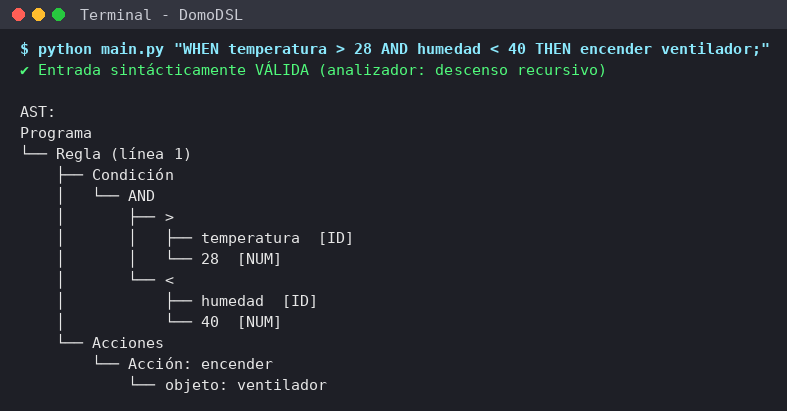
\includegraphics[width=0.78\textwidth]{../docs/img/cap_valida.png}
\caption{Entrada válida: se informa el resultado y se imprime el AST.}
\end{figure}
\begin{figure}[H]\centering
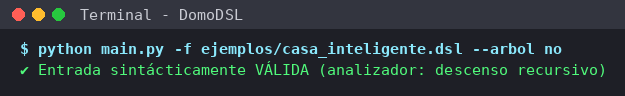
\includegraphics[width=0.95\textwidth]{../docs/img/cap_archivo.png}
\caption{Análisis de un archivo con cuatro reglas (\texttt{ejemplos/casa\_inteligente.dsl}).}
\end{figure}
\begin{figure}[H]\centering
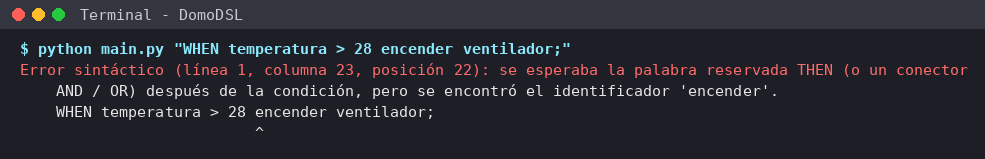
\includegraphics[width=0.95\textwidth]{../docs/img/cap_error_then.png}
\caption{Error sintáctico: falta \texttt{THEN}.}
\end{figure}
\begin{figure}[H]\centering
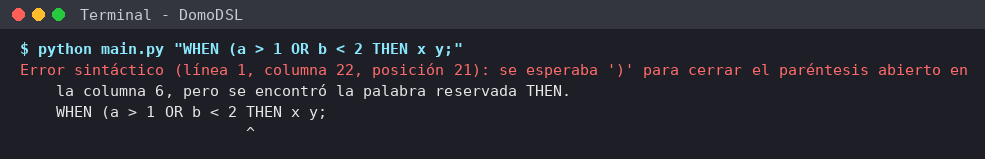
\includegraphics[width=0.95\textwidth]{../docs/img/cap_error_parentesis.png}
\caption{Error sintáctico: paréntesis sin cerrar.}
\end{figure}
\begin{figure}[H]\centering
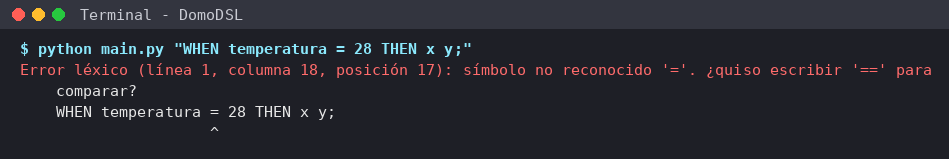
\includegraphics[width=0.95\textwidth]{../docs/img/cap_error_lexico.png}
\caption{Error léxico: \texttt{=} en lugar de \texttt{==}.}
\end{figure}
\begin{figure}[H]\centering
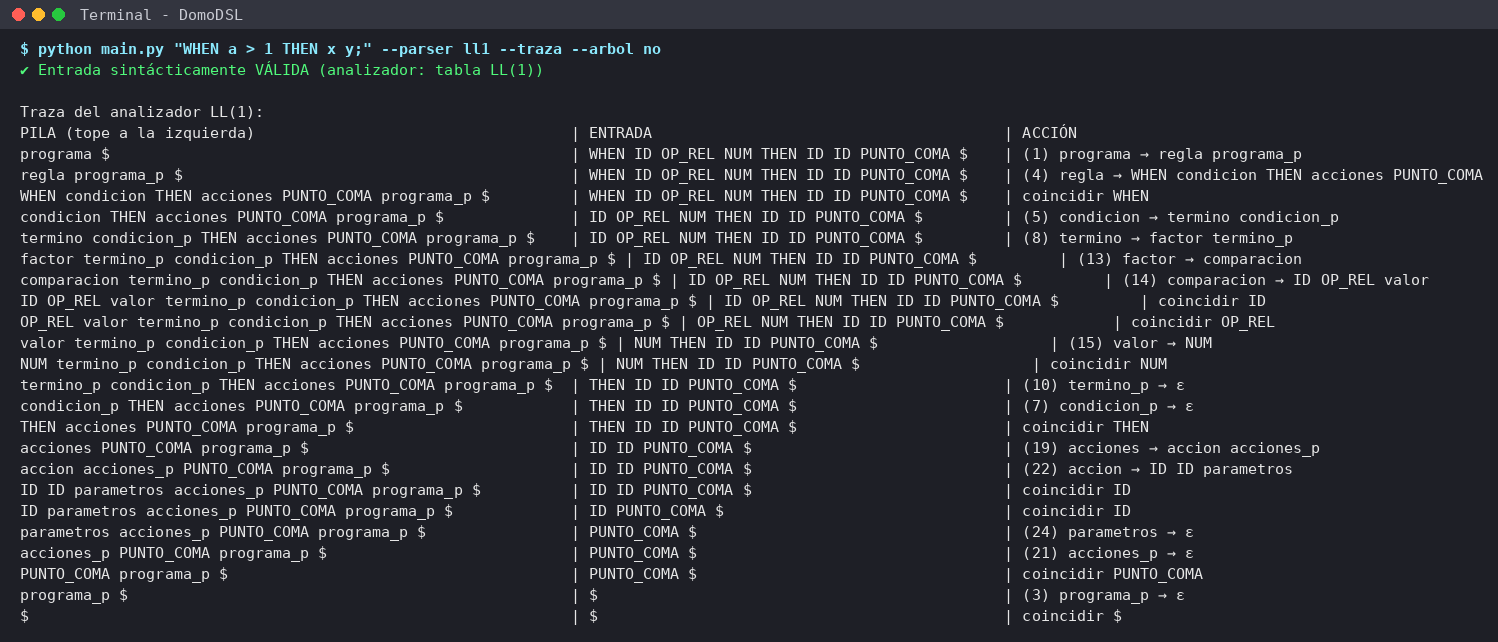
\includegraphics[width=\textwidth]{../docs/img/cap_traza_ll1.png}
\caption{Traza del analizador LL(1) (\texttt{--traza}): pila, entrada restante y producción aplicada.}
\end{figure}
\begin{figure}[H]\centering
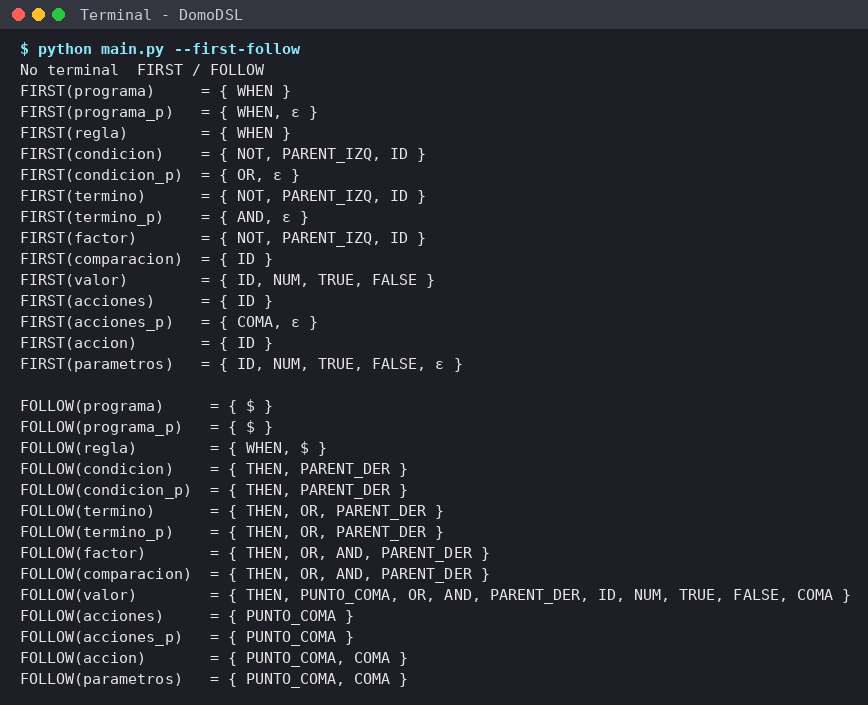
\includegraphics[width=0.85\textwidth]{../docs/img/cap_first_follow.png}
\caption{FIRST y FOLLOW calculados por el programa (\texttt{--first-follow}).}
\end{figure}
\begin{figure}[H]\centering
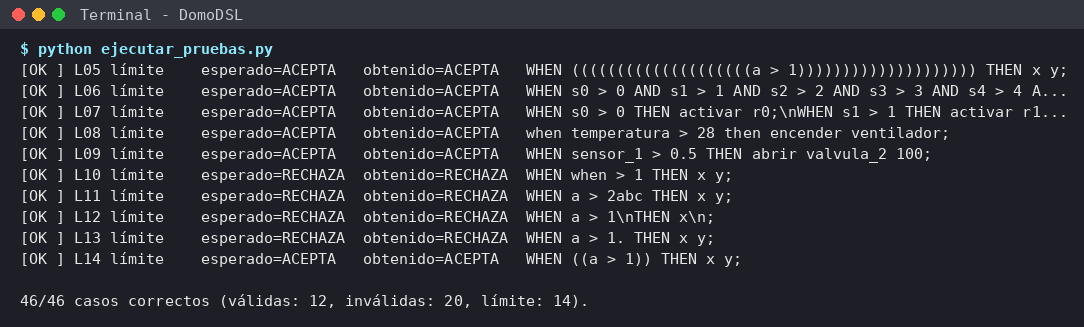
\includegraphics[width=0.95\textwidth]{../docs/img/cap_pruebas.png}
\caption{Resultado de \texttt{ejecutar\_pruebas.py}.}
\end{figure}
\begin{figure}[H]\centering
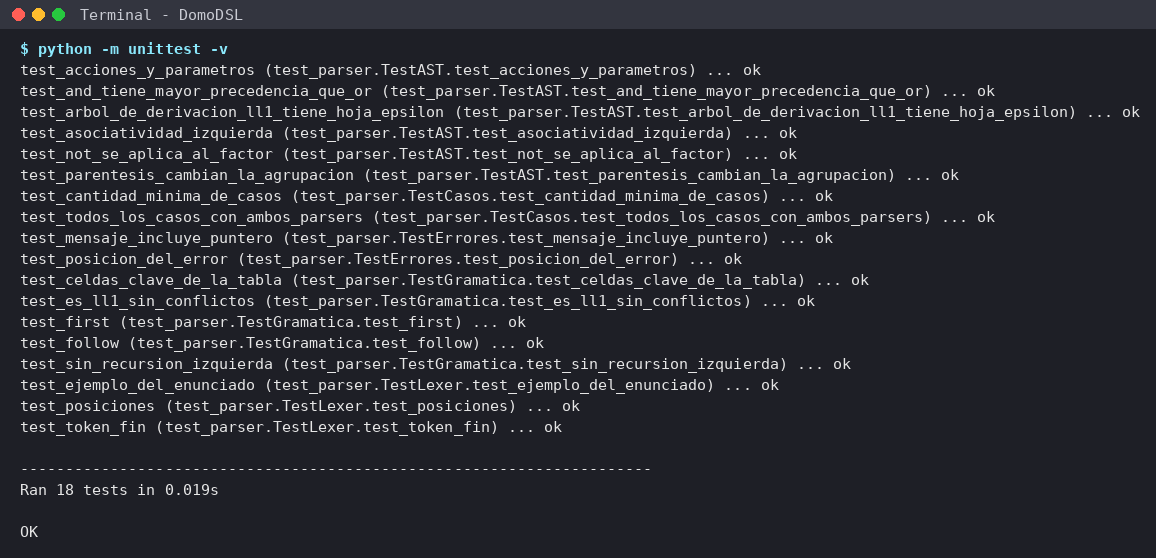
\includegraphics[width=0.95\textwidth]{../docs/img/cap_unittest.png}
\caption{Resultado de las pruebas unitarias.}
\end{figure}

\clearpage
\subsection*{Anexo C. Código fuente de los módulos principales}
\lstinputlisting[caption={lexer.py --- analizador léxico}]{../lexer.py}
\lstinputlisting[caption={gramatica.py --- GLC, FIRST, FOLLOW y tabla LL(1)}]{../gramatica.py}
\lstinputlisting[caption={parser\_rd.py --- parser por descenso recursivo}]{../parser_rd.py}
\lstinputlisting[caption={parser\_ll1.py --- parser dirigido por tabla LL(1)}]{../parser_ll1.py}

\fi
   % seccion 1 (parte 1)
% Sección 2 (tarea C1) - autor: Persona C. Editar solo este archivo.
\section{Especificación del lenguaje}

\subsection{Propósito}
DomoDSL permite escribir programas formados por una o más \textbf{reglas de automatización}. Cada regla evalúa una
\textbf{condición} sobre variables del hogar (temperatura, humedad, movimiento, hora, \dots) y, si se cumple, ordena
una o más \textbf{acciones} sobre dispositivos (ventilador, alarma, termostato, \dots). El lenguaje no ejecuta las
reglas: el objetivo del proyecto es \emph{reconocerlas} (decidir si son sintácticamente válidas), informar errores
útiles y producir una representación estructurada (AST).

\subsection{Alfabeto}
El alfabeto relevante $\Sigma$ está formado por:
\begin{itemize}[nosep]
\item letras \texttt{A--Z} y \texttt{a--z}, dígitos \texttt{0--9}, el guion bajo \texttt{\_} y el punto \texttt{.} (solo dentro de números decimales);
\item los símbolos \texttt{>}, \texttt{<}, \texttt{=}, \texttt{!}, \texttt{;}, \texttt{,}, \texttt{(} y \texttt{)};
\item espacio, tabulación y salto de línea (separadores que el lexer descarta).
\end{itemize}
Cualquier otro carácter produce un \emph{error léxico}.

\subsection{Categorías de tokens}
El analizador léxico (basado en el entregado por el docente) usa expresiones regulares. Los espacios se descartan.
Las palabras reservadas \textbf{no distinguen mayúsculas de minúsculas} (como en la función base).

\begin{center}\small
\begin{tabular}{@{}>{\raggedright\arraybackslash}p{2.5cm} >{\raggedright\arraybackslash}p{4.0cm} >{\raggedright\arraybackslash}p{4.3cm} >{\raggedright\arraybackslash}p{3.3cm}@{}}
\toprule
\textbf{Token} & \textbf{Patrón} & \textbf{Descripción} & \textbf{Ejemplos} \\
\midrule
\texttt{WHEN, THEN} & \texttt{WHEN | THEN} & Inicio y separador de la regla & \texttt{WHEN, then} \\
\texttt{AND, OR, NOT} & \texttt{AND | OR | NOT} & Operadores lógicos & \texttt{AND, not} \\
\texttt{TRUE, FALSE} & \texttt{TRUE | FALSE} & Valores booleanos & \texttt{TRUE} \\
\texttt{ID} & \texttt{[A-Za-z\_][A-Za-z0-9\_]*} & Identificadores (variables, verbos y dispositivos) & \texttt{temperatura, sensor\_1} \\
\texttt{NUM} & \texttt{\textbackslash{}d+(\textbackslash{}.\textbackslash{}d+)?} & Números enteros o decimales & \texttt{28, 0.5} \\
\texttt{OP\_REL} & \texttt{>= | <= | == | != | > | <} & Operadores relacionales & \texttt{>=, ==} \\
\texttt{PUNTO\_COMA} & \texttt{;} & Fin de regla & \texttt{;} \\
\texttt{COMA} & \texttt{,} & Separador de acciones & \texttt{,} \\
\texttt{PARENT\_IZQ} & \texttt{(} & Abre agrupación & \texttt{(} \\
\texttt{PARENT\_DER} & \texttt{)} & Cierra agrupación & \texttt{)} \\
\bottomrule
\end{tabular}
\end{center}

Un identificador cuyo texto coincide con una palabra reservada se convierte en el token reservado
(p.\,ej. \texttt{when} $\to$ \texttt{WHEN}), por lo que las palabras reservadas no pueden usarse como identificadores.
Al final de la entrada el lexer agrega el token \texttt{\$} (fin de entrada), que necesita el analizador LL(1).

\subsection{Cumplimiento de los requisitos mínimos del enunciado}
\begin{center}\small
\begin{tabular}{@{}>{\raggedright\arraybackslash}p{5.6cm} >{\raggedright\arraybackslash}p{9.4cm}@{}}
\toprule
\textbf{Requisito} & \textbf{Cómo lo cumple DomoDSL} \\
\midrule
Al menos 4 palabras reservadas & 7: \texttt{WHEN}, \texttt{THEN}, \texttt{AND}, \texttt{OR}, \texttt{NOT}, \texttt{TRUE}, \texttt{FALSE} \\
Identificadores & Token \texttt{ID} \\
Valores numéricos y/o booleanos & \texttt{NUM} (enteros y decimales) y \texttt{TRUE}/\texttt{FALSE} \\
Al menos 3 operadores & 9: seis relacionales (\texttt{> < >= <= == !=}) y tres lógicos (\texttt{AND OR NOT}) \\
Estructura de sentencia principal & \texttt{WHEN <condición> THEN <acciones> ;} \\
Más de una sentencia & Un programa es una secuencia de una o más reglas \\
Construcción compuesta & Conectores \texttt{AND}/\texttt{OR}, paréntesis y listas de acciones con parámetros \\
Extensión creativa & \texttt{NOT}, paréntesis, múltiples acciones y acciones con parámetros (sección~4.6) \\
\bottomrule
\end{tabular}
\end{center}

\subsection{Ejemplos de sentencias válidas e inválidas}
\paragraph{Válidas.}
\begin{enumerate}[nosep]
\item \texttt{WHEN temperatura > 28 THEN encender ventilador;}
\item \texttt{WHEN movimiento == TRUE THEN activar alarma;}
\item \texttt{WHEN temperatura > 28 AND humedad < 40 THEN encender ventilador;}
\item \texttt{WHEN luz < 100 OR hora >= 20 THEN encender lampara;}
\item \texttt{WHEN NOT puerta == TRUE THEN activar alarma;}
\item \texttt{WHEN (temperatura > 30 OR humedad > 80) AND presencia == TRUE THEN encender aire;}
\item \texttt{WHEN temperatura > 28 THEN encender ventilador 3, activar alarma;}
\end{enumerate}
\paragraph{Inválidas.}
\begin{center}\small
\begin{tabular}{@{}l >{\raggedright\arraybackslash}p{7.2cm} >{\raggedright\arraybackslash}p{6.3cm}@{}}
\toprule
\textbf{N.º} & \textbf{Sentencia} & \textbf{Motivo} \\
\midrule
1 & \texttt{WHEN temperatura > 28 encender ventilador;} & Falta la palabra reservada \texttt{THEN} \\
2 & \texttt{WHEN temperatura > THEN encender ventilador;} & Falta el valor después de \texttt{>} \\
3 & \texttt{temperatura > 28 THEN encender ventilador;} & La regla no comienza con \texttt{WHEN} \\
4 & \texttt{WHEN temperatura > 28 THEN encender ventilador} & Falta el \texttt{;} final \\
5 & \texttt{WHEN (temperatura > 28 THEN encender ventilador;} & Paréntesis sin cerrar \\
6 & \texttt{WHEN temperatura = 28 THEN encender ventilador;} & \texttt{=} no es un operador (debe ser \texttt{==}): error léxico \\
\bottomrule
\end{tabular}
\end{center}


% Secciones 3 a 6: GLC, análisis, FIRST/FOLLOW, tabla LL(1) (tarea R1) - autor: Persona B.
\section{Gramática libre de contexto}

La gramática de DomoDSL es $G = (N, T, P, S)$ con:
\begin{itemize}[nosep]
\item \textbf{No terminales} $N$ (14): \textit{programa}, \textit{programa}$'$, \textit{regla}, \textit{condicion}, \textit{condicion}$'$, \textit{termino}, \textit{termino}$'$, \textit{factor}, \textit{comparacion}, \textit{valor}, \textit{acciones}, \textit{acciones}$'$, \textit{accion}, \textit{parametros}.
\item \textbf{Terminales} $T$ (14, son los tokens): \texttt{WHEN}, \texttt{THEN}, \texttt{PUNTO\_COMA}, \texttt{OR}, \texttt{AND}, \texttt{NOT}, \texttt{PARENT\_IZQ}, \texttt{PARENT\_DER}, \texttt{ID}, \texttt{OP\_REL}, \texttt{NUM}, \texttt{TRUE}, \texttt{FALSE}, \texttt{COMA}.
\item \textbf{Símbolo inicial} $S$ = \textit{programa}.
\item \textbf{Producciones} $P$: las 24 que muestra la tabla siguiente. (Las producciones numeradas son las que usa el
código; el símbolo \textit{x}$'$ se escribe \texttt{x\_p} en el programa.)
\end{itemize}

\begin{longtable}{@{}r p{11cm}@{}}
\toprule
\textbf{N.º} & \textbf{Producción} \\
\midrule
\endhead
1 & \textit{programa} $\rightarrow$ \textit{regla} \textit{programa}$'$ \\
2 & \textit{programa}$'$ $\rightarrow$ \textit{regla} \textit{programa}$'$ \\
3 & \textit{programa}$'$ $\rightarrow$ $\varepsilon$ \\
4 & \textit{regla} $\rightarrow$ \texttt{WHEN} \textit{condicion} \texttt{THEN} \textit{acciones} \texttt{PUNTO\_COMA} \\
5 & \textit{condicion} $\rightarrow$ \textit{termino} \textit{condicion}$'$ \\
6 & \textit{condicion}$'$ $\rightarrow$ \texttt{OR} \textit{termino} \textit{condicion}$'$ \\
7 & \textit{condicion}$'$ $\rightarrow$ $\varepsilon$ \\
8 & \textit{termino} $\rightarrow$ \textit{factor} \textit{termino}$'$ \\
9 & \textit{termino}$'$ $\rightarrow$ \texttt{AND} \textit{factor} \textit{termino}$'$ \\
10 & \textit{termino}$'$ $\rightarrow$ $\varepsilon$ \\
11 & \textit{factor} $\rightarrow$ \texttt{NOT} \textit{factor} \\
12 & \textit{factor} $\rightarrow$ \texttt{PARENT\_IZQ} \textit{condicion} \texttt{PARENT\_DER} \\
13 & \textit{factor} $\rightarrow$ \textit{comparacion} \\
14 & \textit{comparacion} $\rightarrow$ \texttt{ID} \texttt{OP\_REL} \textit{valor} \\
15 & \textit{valor} $\rightarrow$ \texttt{NUM} \\
16 & \textit{valor} $\rightarrow$ \texttt{TRUE} \\
17 & \textit{valor} $\rightarrow$ \texttt{FALSE} \\
18 & \textit{valor} $\rightarrow$ \texttt{ID} \\
19 & \textit{acciones} $\rightarrow$ \textit{accion} \textit{acciones}$'$ \\
20 & \textit{acciones}$'$ $\rightarrow$ \texttt{COMA} \textit{accion} \textit{acciones}$'$ \\
21 & \textit{acciones}$'$ $\rightarrow$ $\varepsilon$ \\
22 & \textit{accion} $\rightarrow$ \texttt{ID} \texttt{ID} \textit{parametros} \\
23 & \textit{parametros} $\rightarrow$ \textit{valor} \textit{parametros} \\
24 & \textit{parametros} $\rightarrow$ $\varepsilon$ \\
\bottomrule
\end{longtable}

\paragraph{Lectura de la gramática.}
\begin{itemize}[nosep]
\item Un \textbf{programa} es una o más reglas (1--3). Una \textbf{regla} es \texttt{WHEN condición THEN acciones ;} (4).
\item Las \textbf{condiciones} se estratifican en tres niveles para codificar la precedencia: \textit{condicion} (OR, la menor),
\textit{termino} (AND) y \textit{factor} (NOT, paréntesis y comparaciones, la mayor) (5--13). Una \textbf{comparación} es
\texttt{ID OP\_REL valor} (14) y un \textbf{valor} es un número, un booleano o un identificador (15--18).
\item Las \textbf{acciones} son una lista separada por comas (19--21); cada una es \texttt{verbo dispositivo [parámetros]} (22--24), donde los
parámetros son cero o más valores.
\end{itemize}

\paragraph{Ejemplo de derivación.} Derivación por la izquierda de \texttt{WHEN a > 1 THEN x y;} (los terminales se muestran como
tipos de token: \texttt{ID}, \texttt{OP\_REL}, \texttt{NUM}, \dots). La derivación fue reconstruida a partir de la traza del analizador LL(1).

\begin{longtable}{@{}r r >{\raggedright\arraybackslash}p{12.2cm}@{}}
\toprule
\textbf{Paso} & \textbf{Prod.} & \textbf{Forma sentencial (derivación por la izquierda)} \\
\midrule
\endhead
0 &  & \footnotesize \textit{programa} \\
1 & 1 & $\Rightarrow$ \footnotesize \textit{regla} \textit{programa}$'$ \\
2 & 4 & $\Rightarrow$ \footnotesize \texttt{WHEN} \textit{condicion} \texttt{THEN} \textit{acciones} \texttt{PUNTO\_COMA} \textit{programa}$'$ \\
3 & 5 & $\Rightarrow$ \footnotesize \texttt{WHEN} \textit{termino} \textit{condicion}$'$ \texttt{THEN} \textit{acciones} \texttt{PUNTO\_COMA} \textit{programa}$'$ \\
4 & 8 & $\Rightarrow$ \footnotesize \texttt{WHEN} \textit{factor} \textit{termino}$'$ \textit{condicion}$'$ \texttt{THEN} \textit{acciones} \texttt{PUNTO\_COMA} \textit{programa}$'$ \\
5 & 13 & $\Rightarrow$ \footnotesize \texttt{WHEN} \textit{comparacion} \textit{termino}$'$ \textit{condicion}$'$ \texttt{THEN} \textit{acciones} \texttt{PUNTO\_COMA} \textit{programa}$'$ \\
6 & 14 & $\Rightarrow$ \footnotesize \texttt{WHEN} \texttt{ID} \texttt{OP\_REL} \textit{valor} \textit{termino}$'$ \textit{condicion}$'$ \texttt{THEN} \textit{acciones} \texttt{PUNTO\_COMA} \textit{programa}$'$ \\
7 & 15 & $\Rightarrow$ \footnotesize \texttt{WHEN} \texttt{ID} \texttt{OP\_REL} \texttt{NUM} \textit{termino}$'$ \textit{condicion}$'$ \texttt{THEN} \textit{acciones} \texttt{PUNTO\_COMA} \textit{programa}$'$ \\
8 & 10 & $\Rightarrow$ \footnotesize \texttt{WHEN} \texttt{ID} \texttt{OP\_REL} \texttt{NUM} \textit{condicion}$'$ \texttt{THEN} \textit{acciones} \texttt{PUNTO\_COMA} \textit{programa}$'$ \\
9 & 7 & $\Rightarrow$ \footnotesize \texttt{WHEN} \texttt{ID} \texttt{OP\_REL} \texttt{NUM} \texttt{THEN} \textit{acciones} \texttt{PUNTO\_COMA} \textit{programa}$'$ \\
10 & 19 & $\Rightarrow$ \footnotesize \texttt{WHEN} \texttt{ID} \texttt{OP\_REL} \texttt{NUM} \texttt{THEN} \textit{accion} \textit{acciones}$'$ \texttt{PUNTO\_COMA} \textit{programa}$'$ \\
11 & 22 & $\Rightarrow$ \footnotesize \texttt{WHEN} \texttt{ID} \texttt{OP\_REL} \texttt{NUM} \texttt{THEN} \texttt{ID} \texttt{ID} \textit{parametros} \textit{acciones}$'$ \texttt{PUNTO\_COMA} \textit{programa}$'$ \\
12 & 24 & $\Rightarrow$ \footnotesize \texttt{WHEN} \texttt{ID} \texttt{OP\_REL} \texttt{NUM} \texttt{THEN} \texttt{ID} \texttt{ID} \textit{acciones}$'$ \texttt{PUNTO\_COMA} \textit{programa}$'$ \\
13 & 21 & $\Rightarrow$ \footnotesize \texttt{WHEN} \texttt{ID} \texttt{OP\_REL} \texttt{NUM} \texttt{THEN} \texttt{ID} \texttt{ID} \texttt{PUNTO\_COMA} \textit{programa}$'$ \\
14 & 3 & $\Rightarrow$ \footnotesize \texttt{WHEN} \texttt{ID} \texttt{OP\_REL} \texttt{NUM} \texttt{THEN} \texttt{ID} \texttt{ID} \texttt{PUNTO\_COMA} \\
\bottomrule
\end{longtable}

\section{Análisis de la gramática}

\subsection{Terminales, no terminales y símbolo inicial}
Ya identificados en la sección~3: 14 terminales (los tokens), 14 no terminales y símbolo inicial \textit{programa}.
Los no terminales \textit{programa'}, \textit{condicion'}, \textit{termino'}, \textit{acciones'} son \emph{auxiliares}
introducidos al transformar la gramática; el resto tiene significado propio del dominio.

\subsection{Primera versión de la gramática ($G_0$)}
Al escribir la gramática de forma natural se obtiene:
\begin{lstlisting}[language={},numbers=none]
programa    → regla programa | regla
regla       → WHEN condicion THEN acciones PUNTO_COMA
condicion   → condicion OR condicion | condicion AND condicion
            | NOT condicion | PARENT_IZQ condicion PARENT_DER | comparacion
comparacion → ID OP_REL valor
valor       → NUM | TRUE | FALSE | ID
acciones    → acciones COMA accion | accion
accion      → ID ID parametros
parametros  → parametros valor | ε
\end{lstlisting}
$G_0$ describe el lenguaje deseado, pero \textbf{no sirve para un analizador predictivo}: tiene recursión por la
izquierda, prefijos comunes y es ambigua. A continuación se analiza cada problema.

\subsection{Recursión por la izquierda}
En $G_0$ hay recursión izquierda \emph{directa} en tres no terminales: \textit{condicion} ($\textit{condicion}\to\textit{condicion}\ \texttt{OR}\ \dots$),
\textit{acciones} y \textit{parametros}. Un parser de descenso recursivo entraría en bucle infinito. Se aplica la
transformación estándar $A\to A\alpha\mid\beta \;\Longrightarrow\; A\to\beta A',\ A'\to\alpha A'\mid\varepsilon$:

\begin{center}\small
\begin{tabular}{@{}>{\raggedright\arraybackslash}p{5.2cm} >{\raggedright\arraybackslash}p{7.3cm} >{\raggedright\arraybackslash}p{2.6cm}@{}}
\toprule
\textbf{Original ($G_0$)} & \textbf{Transformado} & \textbf{En la gramática final} \\
\midrule
$\textit{acciones}\to\textit{acciones}\ \texttt{COMA}\ \textit{accion}\mid\textit{accion}$ &
$\textit{acciones}\to\textit{accion}\ \textit{acciones'}$ & prods. 19--21 \\
 & $\textit{acciones'}\to\texttt{COMA}\ \textit{accion}\ \textit{acciones'}\mid\varepsilon$ & \\
$\textit{parametros}\to\textit{parametros}\ \textit{valor}\mid\varepsilon$ &
$\textit{parametros}\to\textit{valor}\ \textit{parametros}\mid\varepsilon$ (recursión por la derecha, equivalente) & prods. 23--24 \\
$\textit{condicion}\to\textit{condicion}\ \texttt{OR}\ \textit{termino}\mid\textit{termino}$ &
$\textit{condicion}\to\textit{termino}\ \textit{condicion'}$ & prods. 5--7 \\
 & $\textit{condicion'}\to\texttt{OR}\ \textit{termino}\ \textit{condicion'}\mid\varepsilon$ & \\
$\textit{termino}\to\textit{termino}\ \texttt{AND}\ \textit{factor}\mid\textit{factor}$ &
$\textit{termino}\to\textit{factor}\ \textit{termino'}$ & prods. 8--10 \\
 & $\textit{termino'}\to\texttt{AND}\ \textit{factor}\ \textit{termino'}\mid\varepsilon$ & \\
\bottomrule
\end{tabular}
\end{center}

\paragraph{Verificación en la gramática final.} No hay recursión izquierda directa (lo comprueba una prueba unitaria: ninguna producción
empieza con su propio lado izquierdo). Tampoco indirecta: las dependencias por el primer símbolo forman cadenas sin ciclos:
\begin{itemize}[nosep]
\item $\textit{programa}\to\textit{regla}\to\texttt{WHEN}$;
\item $\textit{condicion}\to\textit{termino}\to\textit{factor}\to\textit{comparacion}\to\texttt{ID}$;
\item $\textit{acciones}\to\textit{accion}\to\texttt{ID}$.
\end{itemize}
La única recursión de \textit{factor} ($\textit{factor}\to\texttt{NOT}\ \textit{factor}$) empieza con un terminal, por lo que es inofensiva.

\subsection{Factorización por la izquierda}
En $G_0$, \textit{programa} tiene dos alternativas con prefijo común \textit{regla}
($\textit{programa}\to\textit{regla}\ \textit{programa}\mid\textit{regla}$): con un solo token de lookahead no se
puede elegir. Se factoriza: $\textit{programa}\to\textit{regla}\ \textit{programa'}$ con
$\textit{programa'}\to\textit{programa}\mid\varepsilon$; como $\textit{programa}$ empieza con $\textit{regla}$, se
sustituye y queda $\textit{programa'}\to\textit{regla}\ \textit{programa'}\mid\varepsilon$ (prods. 1--3).
En el resto de la gramática las alternativas de un mismo no terminal comienzan con terminales distintos
(p.\,ej. \textit{factor}: \texttt{NOT}, \texttt{PARENT\_IZQ}, \texttt{ID}), por lo que \textbf{no se requiere más factorización}; esto se
confirma formalmente en la sección~6 (conjuntos de selección disjuntos).

\subsection{Ambigüedad}
$G_0$ es \textbf{ambigua}: la cadena \texttt{a > 1 OR b > 2 AND c > 3} tiene dos árboles de derivación, según si la
producción $\textit{condicion}\to\textit{condicion}\ \texttt{OR}\ \textit{condicion}$ o
$\textit{condicion}\to\textit{condicion}\ \texttt{AND}\ \textit{condicion}$ se aplica en la raíz:
\begin{center}
\texttt{(a > 1 OR b > 2) AND c > 3} \quad frente a \quad \texttt{a > 1 OR (b > 2 AND c > 3)}.
\end{center}
Además \texttt{a OR b OR c} puede agruparse a la izquierda o a la derecha (ambigüedad de asociatividad). Esto cambiaría
el significado del programa, así que debe eliminarse en la gramática, no en el código.

\paragraph{Solución.} Se separan los \textbf{niveles de precedencia} (\textit{condicion} para OR, \textit{termino} para AND,
\textit{factor} para NOT/paréntesis/comparación): AND liga más fuerte que OR, y NOT más que AND. Con las producciones
5--13 la cadena anterior tiene un único árbol, el de \texttt{a > 1 OR (b > 2 AND c > 3)}. La asociatividad es
\textbf{izquierda}: el AST se construye en un ciclo que agrupa \texttt{((a OR b) OR c)} (sección~7).
Como además la gramática final es LL(1) (sección~6), es \textbf{no ambigua} (toda gramática LL(1) lo es).
La guía del enunciado (\textit{condicion2} con AND/OR mezclados) no define precedencia entre ambos conectores; la estratificación
usada aquí sí lo hace.

Otro punto revisado: en \textit{accion}, los parámetros son identificadores/valores y podrían confundirse con el
siguiente elemento; no hay ambigüedad porque la lista de parámetros termina siempre en \texttt{;} o \texttt{,}
(FOLLOW(parametros) = \{\texttt{PUNTO\_COMA}, \texttt{COMA}\}, ver sección~5).

\subsection{Extensión creativa y su efecto en la gramática}
La extensión de DomoDSL tiene tres componentes, todos integrados en la gramática, FIRST/FOLLOW, tabla, código y pruebas:
\begin{enumerate}[nosep]
\item \textbf{Negación} \texttt{NOT}: $\textit{factor}\to\texttt{NOT}\ \textit{factor}$ (prod.~11); permite \texttt{NOT NOT x == 1}.
\item \textbf{Agrupación con paréntesis}: $\textit{factor}\to\texttt{PARENT\_IZQ}\ \textit{condicion}\ \texttt{PARENT\_DER}$ (prod.~12); es la que introduce
\texttt{PARENT\_DER} en FOLLOW(\textit{condicion}) y justifica los mensajes ``falta \texttt{)}'' / ``\texttt{)} sobrante''.
\item \textbf{Acciones múltiples con parámetros} (propia del dominio): $\textit{acciones}$ con \texttt{COMA} (prods.~19--21) y
\textit{parametros} (prods.~23--24); p.\,ej. \texttt{ajustar termostato 22 TRUE, activar alarma}.
\end{enumerate}

\section{FIRST y FOLLOW}

\paragraph{Definiciones.} $\mathrm{FIRST}(\alpha)$ es el conjunto de terminales que pueden iniciar una cadena derivada de $\alpha$
(incluye $\varepsilon$ si $\alpha\Rightarrow^{*}\varepsilon$). $\mathrm{FOLLOW}(A)$ es el conjunto de terminales que pueden aparecer
inmediatamente a la derecha de $A$ en alguna forma sentencial (incluye \texttt{\$} si $A$ puede ir al final).

\paragraph{Reglas usadas.}
\begin{enumerate}[nosep]
\item Si $X$ es terminal, $\mathrm{FIRST}(X)=\{X\}$. Si $X\to\varepsilon$, $\varepsilon\in\mathrm{FIRST}(X)$.
\item Si $X\to Y_1Y_2\cdots Y_k$: se agrega $\mathrm{FIRST}(Y_1)\setminus\{\varepsilon\}$; si $Y_1$ es anulable, también $\mathrm{FIRST}(Y_2)\setminus\{\varepsilon\}$, y así sucesivamente; $\varepsilon\in\mathrm{FIRST}(X)$ si todos los $Y_i$ son anulables.
\item \texttt{\$}$\in\mathrm{FOLLOW}(S)$.
\item Si $A\to\alpha B\beta$: $\mathrm{FIRST}(\beta)\setminus\{\varepsilon\}\subseteq\mathrm{FOLLOW}(B)$.
\item Si $A\to\alpha B$ o $A\to\alpha B\beta$ con $\varepsilon\in\mathrm{FIRST}(\beta)$: $\mathrm{FOLLOW}(A)\subseteq\mathrm{FOLLOW}(B)$.
\end{enumerate}
Los conjuntos se calculan iterando hasta alcanzar el punto fijo (\texttt{calcular\_first} y \texttt{calcular\_follow} en
\texttt{gramatica.py}); los resultados coinciden con el cálculo manual justificado en las tablas y están verificados por
pruebas unitarias (\texttt{test\_first}, \texttt{test\_follow}).

\subsection{Conjuntos FIRST}
\begin{longtable}{@{}>{\raggedright\arraybackslash}p{2.6cm} >{\raggedright\arraybackslash}p{5.3cm} >{\raggedright\arraybackslash}p{6.9cm}@{}}
\toprule
\textbf{No terminal} & \textbf{FIRST} & \textbf{Justificación} \\
\midrule
\endhead
\textit{programa} & $\{$ \texttt{WHEN} $\}$ & \footnotesize Prod. 1: empieza por \textit{regla}, que no deriva $\varepsilon$; FIRST(programa) = FIRST(regla). \\
\textit{programa}$'$ & $\{$ \texttt{WHEN}, $\varepsilon$ $\}$ & \footnotesize Prod. 2: FIRST(regla) = \{WHEN\}; prod. 3 aporta $\varepsilon$. \\
\textit{regla} & $\{$ \texttt{WHEN} $\}$ & \footnotesize Prod. 4: empieza con el terminal WHEN. \\
\textit{condicion} & $\{$ \texttt{NOT}, \texttt{PARENT\_IZQ}, \texttt{ID} $\}$ & \footnotesize Prod. 5: \textit{termino} no es anulable, luego FIRST(condicion) = FIRST(termino). \\
\textit{condicion}$'$ & $\{$ \texttt{OR}, $\varepsilon$ $\}$ & \footnotesize Prod. 6 empieza con OR; prod. 7 aporta $\varepsilon$. \\
\textit{termino} & $\{$ \texttt{NOT}, \texttt{PARENT\_IZQ}, \texttt{ID} $\}$ & \footnotesize Prod. 8: \textit{factor} no es anulable, luego FIRST(termino) = FIRST(factor). \\
\textit{termino}$'$ & $\{$ \texttt{AND}, $\varepsilon$ $\}$ & \footnotesize Prod. 9 empieza con AND; prod. 10 aporta $\varepsilon$. \\
\textit{factor} & $\{$ \texttt{NOT}, \texttt{PARENT\_IZQ}, \texttt{ID} $\}$ & \footnotesize Prod. 11: NOT; prod. 12: PARENT\_IZQ; prod. 13: FIRST(comparacion) = \{ID\}. \\
\textit{comparacion} & $\{$ \texttt{ID} $\}$ & \footnotesize Prod. 14: empieza con el terminal ID. \\
\textit{valor} & $\{$ \texttt{ID}, \texttt{NUM}, \texttt{TRUE}, \texttt{FALSE} $\}$ & \footnotesize Prods. 15--18: NUM, TRUE, FALSE e ID. \\
\textit{acciones} & $\{$ \texttt{ID} $\}$ & \footnotesize Prod. 19: FIRST(accion) = \{ID\}; \textit{accion} no es anulable. \\
\textit{acciones}$'$ & $\{$ \texttt{COMA}, $\varepsilon$ $\}$ & \footnotesize Prod. 20 empieza con COMA; prod. 21 aporta $\varepsilon$. \\
\textit{accion} & $\{$ \texttt{ID} $\}$ & \footnotesize Prod. 22: empieza con el terminal ID. \\
\textit{parametros} & $\{$ \texttt{ID}, \texttt{NUM}, \texttt{TRUE}, \texttt{FALSE}, $\varepsilon$ $\}$ & \footnotesize Prod. 23: FIRST(valor); prod. 24 aporta $\varepsilon$. \\
\bottomrule
\end{longtable}

Los no terminales anulables son \textit{programa'}, \textit{condicion'}, \textit{termino'}, \textit{acciones'} y \textit{parametros}.

\subsection{Conjuntos FOLLOW}
\begin{longtable}{@{}>{\raggedright\arraybackslash}p{2.6cm} >{\raggedright\arraybackslash}p{5.3cm} >{\raggedright\arraybackslash}p{6.9cm}@{}}
\toprule
\textbf{No terminal} & \textbf{FOLLOW} & \textbf{Justificación} \\
\midrule
\endhead
\textit{programa} & $\{$ \texttt{\$} $\}$ & \footnotesize Símbolo inicial: se agrega \$. \\
\textit{programa}$'$ & $\{$ \texttt{\$} $\}$ & \footnotesize Prod. 1: \textit{programa'} está al final, luego FOLLOW(programa) $\subseteq$ FOLLOW(programa'); la prod. 2 solo repite la regla. \\
\textit{regla} & $\{$ \texttt{WHEN}, \texttt{\$} $\}$ & \footnotesize Prods. 1 y 2: sigue \textit{programa'}; FIRST(programa')$\setminus\{\varepsilon\}$ = \{WHEN\} y como es anulable se agrega FOLLOW(programa') = \{\$\}. \\
\textit{condicion} & $\{$ \texttt{THEN}, \texttt{PARENT\_DER} $\}$ & \footnotesize Prod. 4: sigue THEN. Prod. 12: sigue PARENT\_DER. \\
\textit{condicion}$'$ & $\{$ \texttt{THEN}, \texttt{PARENT\_DER} $\}$ & \footnotesize Prods. 5 y 6: va al final, luego hereda FOLLOW(condicion). \\
\textit{termino} & $\{$ \texttt{THEN}, \texttt{OR}, \texttt{PARENT\_DER} $\}$ & \footnotesize Prods. 5 y 6: sigue \textit{condicion'}; FIRST = \{OR\} y es anulable, luego se agrega FOLLOW(condicion). \\
\textit{termino}$'$ & $\{$ \texttt{THEN}, \texttt{OR}, \texttt{PARENT\_DER} $\}$ & \footnotesize Prods. 8 y 9: va al final, luego hereda FOLLOW(termino). \\
\textit{factor} & $\{$ \texttt{THEN}, \texttt{OR}, \texttt{AND}, \texttt{PARENT\_DER} $\}$ & \footnotesize Prods. 8 y 9: sigue \textit{termino'}: AND, y por ser anulable FOLLOW(termino). Prod. 11 (NOT factor): hereda FOLLOW(factor) (sin efecto nuevo). \\
\textit{comparacion} & $\{$ \texttt{THEN}, \texttt{OR}, \texttt{AND}, \texttt{PARENT\_DER} $\}$ & \footnotesize Prod. 13: va al final, luego hereda FOLLOW(factor). \\
\textit{valor} & $\{$ \texttt{THEN}, \texttt{PUNTO\_COMA}, \texttt{OR}, \texttt{AND}, \texttt{PARENT\_DER}, \texttt{ID}, \texttt{NUM}, \texttt{TRUE}, \texttt{FALSE}, \texttt{COMA} $\}$ & \footnotesize Prod. 14: va al final, hereda FOLLOW(comparacion). Prod. 23: sigue \textit{parametros}: FIRST(parametros)$\setminus\{\varepsilon\}$ y, al ser anulable, FOLLOW(parametros). \\
\textit{acciones} & $\{$ \texttt{PUNTO\_COMA} $\}$ & \footnotesize Prod. 4: sigue PUNTO\_COMA. \\
\textit{acciones}$'$ & $\{$ \texttt{PUNTO\_COMA} $\}$ & \footnotesize Prods. 19 y 20: va al final, luego hereda FOLLOW(acciones). \\
\textit{accion} & $\{$ \texttt{PUNTO\_COMA}, \texttt{COMA} $\}$ & \footnotesize Prods. 19 y 20: sigue \textit{acciones'}: COMA, y por ser anulable FOLLOW(acciones) (y FOLLOW(acciones')). \\
\textit{parametros} & $\{$ \texttt{PUNTO\_COMA}, \texttt{COMA} $\}$ & \footnotesize Prod. 22: va al final, hereda FOLLOW(accion). Prod. 23: va al final, hereda FOLLOW(parametros). \\
\bottomrule
\end{longtable}

\section{Tabla LL(1)}

\paragraph{Construcción.} Para cada producción $A\to\alpha$ (numerada $n$): (a) para cada terminal $a\in\mathrm{FIRST}(\alpha)\setminus\{\varepsilon\}$,
se escribe $n$ en $M[A,a]$; (b) si $\varepsilon\in\mathrm{FIRST}(\alpha)$, se escribe $n$ en $M[A,b]$ para cada
$b\in\mathrm{FOLLOW}(A)$ (incluido \texttt{\$}). Una celda vacía significa error sintáctico.

\begin{landscape}
\begin{table}[H]
\centering
\caption{Tabla predictiva LL(1) de DomoDSL (cada número es la producción de la sección 3; celda vacía = error).}
\normalsize\setlength{\tabcolsep}{2pt}\renewcommand{\arraystretch}{1.25}
\begin{tabular}{@{}l|>{\centering\arraybackslash}p{1.4cm}>{\centering\arraybackslash}p{1.4cm}>{\centering\arraybackslash}p{1.4cm}>{\centering\arraybackslash}p{1.4cm}>{\centering\arraybackslash}p{1.4cm}>{\centering\arraybackslash}p{1.4cm}>{\centering\arraybackslash}p{1.4cm}>{\centering\arraybackslash}p{1.4cm}>{\centering\arraybackslash}p{1.4cm}>{\centering\arraybackslash}p{1.4cm}>{\centering\arraybackslash}p{1.4cm}>{\centering\arraybackslash}p{1.4cm}>{\centering\arraybackslash}p{1.4cm}>{\centering\arraybackslash}p{1.4cm}>{\centering\arraybackslash}p{1.4cm}@{}}
\toprule
 & {\fontsize{6.5}{7}\selectfont \texttt{WHEN}} & {\fontsize{6.5}{7}\selectfont \texttt{THEN}} & {\fontsize{6.5}{7}\selectfont \texttt{PUNTO\_COMA}} & {\fontsize{6.5}{7}\selectfont \texttt{OR}} & {\fontsize{6.5}{7}\selectfont \texttt{AND}} & {\fontsize{6.5}{7}\selectfont \texttt{NOT}} & {\fontsize{6.5}{7}\selectfont \texttt{PARENT\_IZQ}} & {\fontsize{6.5}{7}\selectfont \texttt{PARENT\_DER}} & {\fontsize{6.5}{7}\selectfont \texttt{ID}} & {\fontsize{6.5}{7}\selectfont \texttt{OP\_REL}} & {\fontsize{6.5}{7}\selectfont \texttt{NUM}} & {\fontsize{6.5}{7}\selectfont \texttt{TRUE}} & {\fontsize{6.5}{7}\selectfont \texttt{FALSE}} & {\fontsize{6.5}{7}\selectfont \texttt{COMA}} & {\fontsize{6.5}{7}\selectfont \texttt{\$}} \\
\midrule
\textit{programa} & \cellcolor{celda}\textbf{1} &  &  &  &  &  &  &  &  &  &  &  &  &  &  \\
\textit{programa}$'$ & \cellcolor{celda}\textbf{2} &  &  &  &  &  &  &  &  &  &  &  &  &  & \cellcolor{celda}\textbf{3} \\
\textit{regla} & \cellcolor{celda}\textbf{4} &  &  &  &  &  &  &  &  &  &  &  &  &  &  \\
\textit{condicion} &  &  &  &  &  & \cellcolor{celda}\textbf{5} & \cellcolor{celda}\textbf{5} &  & \cellcolor{celda}\textbf{5} &  &  &  &  &  &  \\
\textit{condicion}$'$ &  & \cellcolor{celda}\textbf{7} &  & \cellcolor{celda}\textbf{6} &  &  &  & \cellcolor{celda}\textbf{7} &  &  &  &  &  &  &  \\
\textit{termino} &  &  &  &  &  & \cellcolor{celda}\textbf{8} & \cellcolor{celda}\textbf{8} &  & \cellcolor{celda}\textbf{8} &  &  &  &  &  &  \\
\textit{termino}$'$ &  & \cellcolor{celda}\textbf{10} &  & \cellcolor{celda}\textbf{10} & \cellcolor{celda}\textbf{9} &  &  & \cellcolor{celda}\textbf{10} &  &  &  &  &  &  &  \\
\textit{factor} &  &  &  &  &  & \cellcolor{celda}\textbf{11} & \cellcolor{celda}\textbf{12} &  & \cellcolor{celda}\textbf{13} &  &  &  &  &  &  \\
\textit{comparacion} &  &  &  &  &  &  &  &  & \cellcolor{celda}\textbf{14} &  &  &  &  &  &  \\
\textit{valor} &  &  &  &  &  &  &  &  & \cellcolor{celda}\textbf{18} &  & \cellcolor{celda}\textbf{15} & \cellcolor{celda}\textbf{16} & \cellcolor{celda}\textbf{17} &  &  \\
\textit{acciones} &  &  &  &  &  &  &  &  & \cellcolor{celda}\textbf{19} &  &  &  &  &  &  \\
\textit{acciones}$'$ &  &  & \cellcolor{celda}\textbf{21} &  &  &  &  &  &  &  &  &  &  & \cellcolor{celda}\textbf{20} &  \\
\textit{accion} &  &  &  &  &  &  &  &  & \cellcolor{celda}\textbf{22} &  &  &  &  &  &  \\
\textit{parametros} &  &  & \cellcolor{celda}\textbf{24} &  &  &  &  &  & \cellcolor{celda}\textbf{23} &  & \cellcolor{celda}\textbf{23} & \cellcolor{celda}\textbf{23} & \cellcolor{celda}\textbf{23} & \cellcolor{celda}\textbf{24} &  \\
\bottomrule
\end{tabular}
\end{table}
\end{landscape}

\subsection{¿Es la gramática LL(1)?}
\textbf{Sí.} Ninguna celda contiene más de una producción (el programa lo verifica: \texttt{CONFLICTOS = []}).
Equivalentemente, para cada no terminal con varias alternativas los \emph{conjuntos de selección}
$\mathrm{SEL}(A\to\alpha)=\mathrm{FIRST}(\alpha)\setminus\{\varepsilon\}\ \cup\ (\mathrm{FOLLOW}(A)\text{ si }\varepsilon\in\mathrm{FIRST}(\alpha))$
son disjuntos de a pares:

\begin{longtable}{@{}>{\raggedright\arraybackslash}p{2.3cm} >{\raggedright\arraybackslash}p{4.0cm} >{\raggedright\arraybackslash}p{5.9cm} c@{}}
\toprule
\textbf{No terminal} & \textbf{Producción} & \textbf{Conjunto de selección} & \textbf{¿Disjuntos?} \\
\midrule
\endhead
\textit{programa}$'$ & (2)  \textit{regla} \textit{programa}$'$ & $\{$ \texttt{WHEN} $\}$ & \textbf{sí} \\
 & (3)  $\varepsilon$ & $\{$ \texttt{\$} $\}$ &  \\
\midrule
\textit{condicion}$'$ & (6)  \texttt{OR} \textit{termino} \textit{condicion}$'$ & $\{$ \texttt{OR} $\}$ & \textbf{sí} \\
 & (7)  $\varepsilon$ & $\{$ \texttt{THEN}, \texttt{PARENT\_DER} $\}$ &  \\
\midrule
\textit{termino}$'$ & (9)  \texttt{AND} \textit{factor} \textit{termino}$'$ & $\{$ \texttt{AND} $\}$ & \textbf{sí} \\
 & (10)  $\varepsilon$ & $\{$ \texttt{THEN}, \texttt{OR}, \texttt{PARENT\_DER} $\}$ &  \\
\midrule
\textit{factor} & (11)  \texttt{NOT} \textit{factor} & $\{$ \texttt{NOT} $\}$ & \textbf{sí} \\
 & (12)  \texttt{PARENT\_IZQ} \textit{condicion} \texttt{PARENT\_DER} & $\{$ \texttt{PARENT\_IZQ} $\}$ &  \\
 & (13)  \textit{comparacion} & $\{$ \texttt{ID} $\}$ &  \\
\midrule
\textit{valor} & (15)  \texttt{NUM} & $\{$ \texttt{NUM} $\}$ & \textbf{sí} \\
 & (16)  \texttt{TRUE} & $\{$ \texttt{TRUE} $\}$ &  \\
 & (17)  \texttt{FALSE} & $\{$ \texttt{FALSE} $\}$ &  \\
 & (18)  \texttt{ID} & $\{$ \texttt{ID} $\}$ &  \\
\midrule
\textit{acciones}$'$ & (20)  \texttt{COMA} \textit{accion} \textit{acciones}$'$ & $\{$ \texttt{COMA} $\}$ & \textbf{sí} \\
 & (21)  $\varepsilon$ & $\{$ \texttt{PUNTO\_COMA} $\}$ &  \\
\midrule
\textit{parametros} & (23)  \textit{valor} \textit{parametros} & $\{$ \texttt{ID}, \texttt{NUM}, \texttt{TRUE}, \texttt{FALSE} $\}$ & \textbf{sí} \\
 & (24)  $\varepsilon$ & $\{$ \texttt{PUNTO\_COMA}, \texttt{COMA} $\}$ &  \\
\bottomrule
\end{longtable}

\paragraph{Puntos delicados y por qué no hay conflicto.}
\begin{itemize}[nosep]
\item \textit{parametros}: las producciones $\textit{valor}\ \textit{parametros}$ (selección $\{\texttt{NUM},\texttt{TRUE},\texttt{FALSE},\texttt{ID}\}$) y $\varepsilon$ (selección
$\mathrm{FOLLOW}=\{\texttt{PUNTO\_COMA},\texttt{COMA}\}$) no se solapan, precisamente porque la lista de parámetros siempre termina en
\texttt{;} o \texttt{,}.
\item \textit{termino'} y \textit{condicion'}: la alternativa vacía se elige con $\mathrm{FOLLOW}$ (\texttt{OR}, \texttt{THEN}, \texttt{)}), que no
contiene \texttt{AND}; por eso AND se asocia siempre antes que OR (precedencia).
\item \textit{programa'}: \texttt{WHEN} inicia otra regla y \texttt{\$} termina el programa.
\end{itemize}
\paragraph{Conclusión.} No fue necesario modificar la gramática después de calcular la tabla: las transformaciones de la
sección~4 ya dejaron una gramática LL(1) utilizable por ambos analizadores.


% Secciones 7 a 9: parser, AST, errores (tarea R2) - autor: Persona A.
\section{Diseño e implementación del parser}

\subsection{Arquitectura}
\begin{center}\small
\begin{tabular}{@{}>{\raggedright\arraybackslash}p{4.4cm} >{\raggedright\arraybackslash}p{10.2cm}@{}}
\toprule
\textbf{Módulo} & \textbf{Responsabilidad} \\
\midrule
\texttt{lexer.py} & Texto $\to$ lista de \texttt{Token} (tipo, lexema, posición, línea, columna) terminada en \texttt{\$}. Error léxico para símbolos desconocidos. \\
\texttt{gramatica.py} & Lista \texttt{PRODUCCIONES}; \texttt{calcular\_first}, \texttt{calcular\_follow}, \texttt{construir\_tabla}; detección de conflictos. \\
\texttt{parser\_rd.py} & Parser predictivo por \textbf{descenso recursivo}; construye el \textbf{AST}. \\
\texttt{parser\_ll1.py} & Parser \textbf{dirigido por la tabla LL(1)} con pila; construye el árbol de derivación y una traza. \\
\texttt{arbol.py} & Clases del AST, árbol genérico, texto jerárquico y exportación a Graphviz. \\
\texttt{errores.py} & \texttt{ErrorLexico} y \texttt{ErrorSintactico} (mensaje, posición, línea, columna, puntero \texttt{\^{}}). \\
\texttt{main.py} & Interfaz de línea de comandos (archivo, texto, modo interactivo, opciones de visualización). \\
\texttt{casos\_prueba.py}, \texttt{ejecutar\_pruebas.py}, \texttt{test\_parser.py} & Casos, ejecutor con ambos parsers y pruebas unitarias. \\
\bottomrule
\end{tabular}
\end{center}
Ningún módulo usa bibliotecas de generación de parsers: solo la biblioteca estándar de Python
(\texttt{re}, \texttt{dataclasses}, \texttt{argparse}, \dots).

\subsection{Analizador léxico}
Parte de la función \texttt{analizador\_lexico} entregada por el docente (expresiones regulares nombradas combinadas en un patrón único).
Se ampliaron: el token \texttt{COMA}; números decimales; el \textbf{registro de posición} (offset, línea y columna) de cada token,
necesario para ubicar los errores; el token de fin \texttt{\$}; y mensajes léxicos con sugerencia (``¿quiso escribir \texttt{==}?'').

\subsection{Parser por descenso recursivo}
Hay \textbf{un método por cada no terminal}, y cada método implementa sus producciones; los comentarios del código indican el
número de producción. Los no terminales auxiliares (\textit{programa'}, \textit{condicion'}, \textit{termino'}, \textit{acciones'},
\textit{parametros}) se implementan como ciclos \texttt{while}, que equivalen a la recursión por la derecha de la gramática
pero (i)~no desbordan la pila de Python con programas largos y (ii)~permiten construir el AST con asociatividad izquierda.
Cuando la alternativa elegida es $\varepsilon$, el parser verifica que el lookahead pertenezca a FOLLOW del no terminal, para
informar el error en el punto exacto en que aparece.

\begin{center}\small
\begin{tabular}{@{}>{\raggedright\arraybackslash}p{6cm} >{\raggedright\arraybackslash}p{9.3cm}@{}}
\toprule
\textbf{Producciones} & \textbf{Método (\texttt{ParserDescendente})} \\
\midrule
1--3 \;(\textit{programa}, \textit{programa'}) & \texttt{programa()} \\
4 \;(\textit{regla}) & \texttt{regla()} \\
5--7 \;(\textit{condicion}, \textit{condicion'}) & \texttt{condicion()} --- ciclo \texttt{while OR} \\
8--10 \;(\textit{termino}, \textit{termino'}) & \texttt{termino()} --- ciclo \texttt{while AND} + verificación FOLLOW \\
11--13 \;(\textit{factor}) & \texttt{factor()} \\
14 \;(\textit{comparacion}) & \texttt{comparacion()} \\
15--18 \;(\textit{valor}) & \texttt{valor()} \\
19--21 \;(\textit{acciones}, \textit{acciones'}) & \texttt{acciones()} --- ciclo \texttt{while COMA} \\
22--24 \;(\textit{accion}, \textit{parametros}) & \texttt{accion()} --- ciclo \texttt{while} lookahead $\in$ FIRST(valor) \\
\bottomrule
\end{tabular}
\end{center}

\lstinputlisting[firstline=105, lastline=151, firstnumber=105, caption={Extracto de parser\_rd.py: condicion, termino y factor (niveles de precedencia).}]{../parser_rd.py}

\subsection{Parser dirigido por tabla LL(1)}
El segundo analizador usa la \emph{misma} lista de producciones: la tabla se genera automáticamente desde \texttt{gramatica.py} y se
interpreta con una pila (inicializada con \texttt{\$ programa}). Si el tope es un terminal, debe coincidir con el token actual; si es un
no terminal, se consulta $M[X,a]$, se reemplaza $X$ por el lado derecho de la producción (en orden inverso) y se agregan los
nodos hijos al árbol de derivación. Una celda vacía produce un error que lista los terminales esperados (la fila de la tabla).
La opción \texttt{--traza} imprime cada paso (pila, entrada restante, acción); ver la captura del Anexo~B.

\lstinputlisting[firstline=47, lastline=87, firstnumber=47, caption={Extracto de parser\_ll1.py: bucle principal del analizador LL(1).}]{../parser_ll1.py}

\subsection{Coherencia entre gramática, informe y código}
La lista \texttt{PRODUCCIONES} es la \emph{única} fuente de verdad: de ella salen FIRST, FOLLOW, la tabla, el parser LL(1) y las tablas de este
informe (generadas por \texttt{informe/generar\_informe.py}). El parser por descenso recursivo se escribió a mano siguiendo cada
producción, y la suite de pruebas comprueba que ambos analizadores aceptan y rechazan exactamente las mismas entradas
(46 casos).

\section{Árbol sintáctico / AST}

El sistema construye dos representaciones:
\begin{itemize}[nosep]
\item \textbf{Árbol de derivación} (concreto), generado por el parser LL(1): contiene todos los no terminales, incluidos los auxiliares y las hojas $\varepsilon$.
\item \textbf{AST} (abstracto), generado por el parser de descenso recursivo: elimina los no terminales auxiliares, los paréntesis y las hojas $\varepsilon$; los
operadores son nodos internos y la asociatividad izquierda queda explícita (\texttt{Or(Or(a,b),c)}).
\end{itemize}
Ambos pueden mostrarse como texto jerárquico o exportarse a Graphviz (\texttt{--dot}).

\subsection{AST de la regla del enunciado}
Entrada: \texttt{WHEN temperatura > 28 AND humedad < 40 THEN encender ventilador;}
{\small
\begin{verbatim}
Programa
└── Regla (línea 1)
    ├── Condición
    │   └── AND
    │       ├── >
    │       │   ├── temperatura  [ID]
    │       │   └── 28  [NUM]
    │       └── <
    │           ├── humedad  [ID]
    │           └── 40  [NUM]
    └── Acciones
        └── Acción: encender
            └── objeto: ventilador
\end{verbatim}}
\begin{figure}[H]
\centering
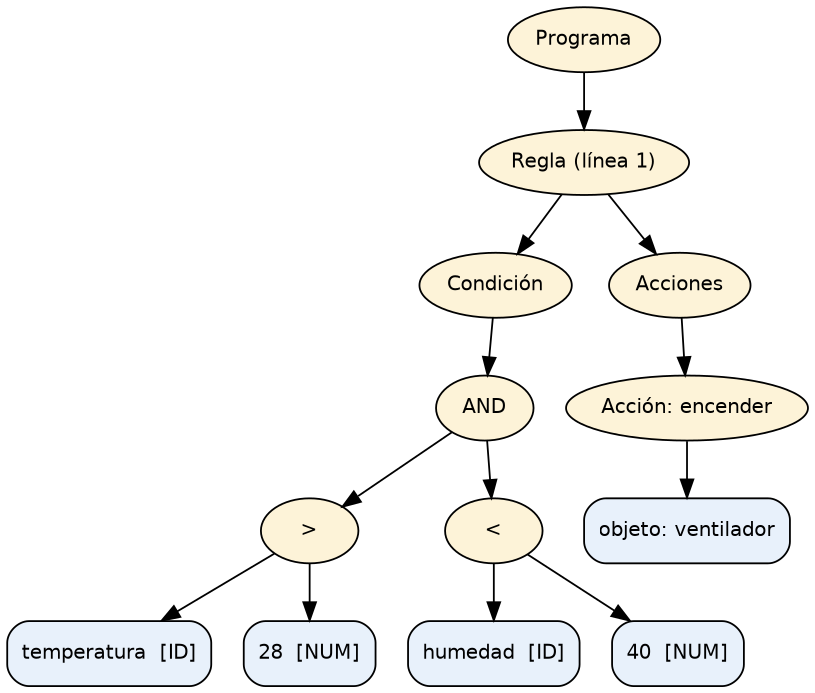
\includegraphics[width=0.55\textwidth]{../docs/img/ast_enunciado.png}
\caption{AST generado (Graphviz) para la regla del enunciado. Óvalos: nodos internos; cajas: hojas.}
\end{figure}

\subsection{AST con la extensión (NOT, paréntesis, acciones múltiples con parámetros)}
Entrada: \texttt{WHEN NOT (puerta == TRUE) AND (hora >= 22 OR hora < 6) THEN bloquear puerta\_principal, ajustar termostato 22;}

Se observa que el AST refleja la precedencia (\texttt{AND} es la raíz de la condición; \texttt{OR} queda dentro del segundo operando por los paréntesis)
y que los paréntesis no aparecen como nodos: su efecto está en la forma del árbol.
\begin{figure}[H]
\centering
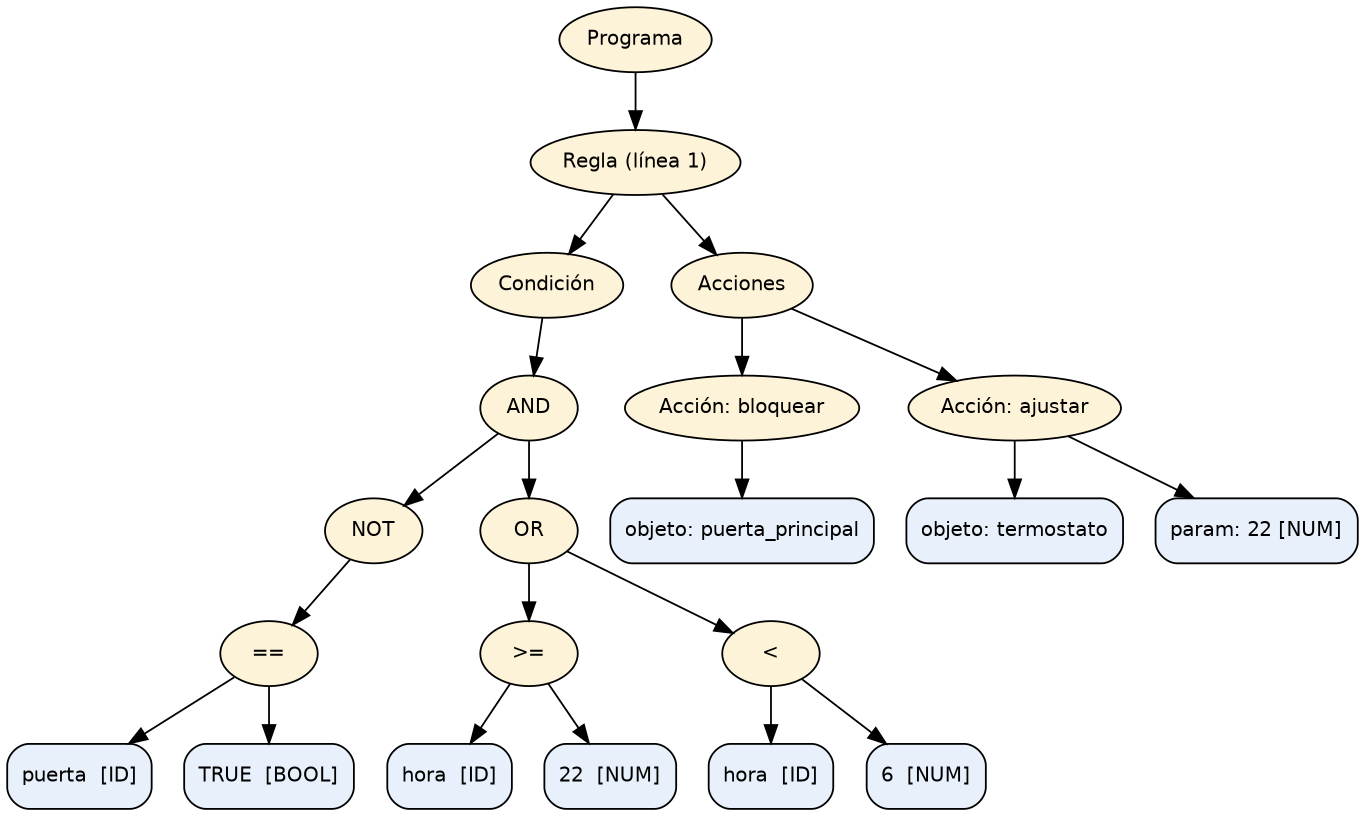
\includegraphics[width=\textwidth]{../docs/img/ast_extension.png}
\caption{AST de una regla con \texttt{NOT}, paréntesis, dos acciones y un parámetro.}
\end{figure}

\subsection{Árbol de derivación (parser LL(1))}
Para \texttt{WHEN a > 1 THEN x y;}; las hojas $\varepsilon$ corresponden a las producciones vacías 3, 7, 10, 21 y 24.
\begin{figure}[H]
\centering
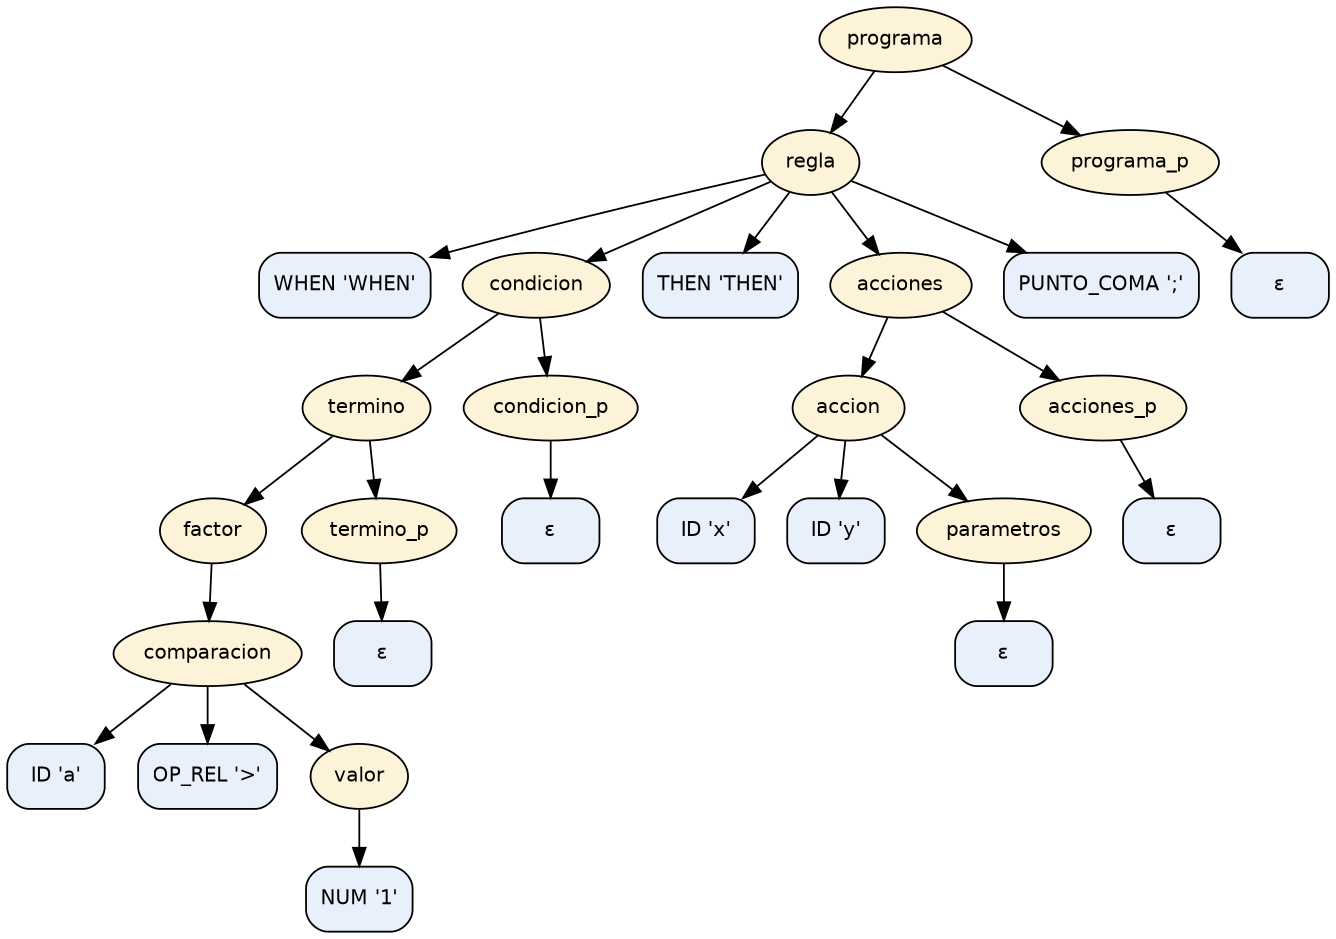
\includegraphics[width=\textwidth]{../docs/img/derivacion_simple.png}
\caption{Árbol de derivación obtenido con la tabla LL(1).}
\end{figure}

\section{Manejo de errores}

\paragraph{Estrategia.} El analizador se detiene en el \textbf{primer error} y lo informa con tres datos de ubicación
(línea, columna y posición/offset), el mensaje, la línea de código afectada y un puntero \texttt{\^{}} bajo el token problemático.
Hay dos clases de error: \texttt{ErrorLexico} (carácter fuera del alfabeto) y \texttt{ErrorSintactico}.
Los mensajes siguen el formato \emph{se esperaba} $X$ \emph{[contexto]}, \emph{pero se encontró} $Y$, y dependen del contexto sintáctico:
\begin{itemize}[nosep]
\item Después de la condición se pide \texttt{THEN} (o un conector AND/OR) y, dentro de un paréntesis, se pide \texttt{)} indicando la columna donde se abrió.
\item Un \texttt{)} sin \texttt{(} se informa como ``paréntesis de cierre sin su \texttt{(} correspondiente''.
\item Cada punto de la gramática tiene su mensaje: valor tras el operador, operador tras el identificador, dispositivo tras la acción, \texttt{;} al final, etc.
\item La entrada vacía tiene un mensaje propio.
\end{itemize}
La notación $[l{:}c]$ indica línea y columna. En el programa, el mensaje completo incluye también la posición (offset).

\subsection{Mensajes del analizador de descenso recursivo}
\begin{longtable}{@{}l >{\raggedright\arraybackslash}p{5.2cm} >{\raggedright\arraybackslash}p{8.4cm}@{}}
\toprule
\textbf{Caso} & \textbf{Entrada} & \textbf{Mensaje entregado por el analizador} \\
\midrule
\endhead
I01 & \footnotesize \texttt{WHEN temperatura > 28 encender ventilador;} & \footnotesize Error sintáctico [1:23]: se esperaba la palabra reservada THEN (o un conector AND / OR) después de la condición, pero se encontró el identificador 'encender'. \\
\addlinespace[2pt]
I02 & \footnotesize \texttt{WHEN temperatura > THEN encender ventilador;} & \footnotesize Error sintáctico [1:20]: se esperaba un valor (número, TRUE, FALSE o identificador) después del operador >, pero se encontró la palabra reservada THEN. \\
\addlinespace[2pt]
I03 & \footnotesize \texttt{WHEN temperatura 28 THEN encender ventilador;} & \footnotesize Error sintáctico [1:18]: se esperaba un operador relacional ('>', '<', '>=', '<=', '==', '!=') después de 'temperatura', pero se encontró el número 28. \\
\addlinespace[2pt]
I05 & \footnotesize \texttt{WHEN temperatura > 28 THEN encender ventilador} & \footnotesize Error sintáctico [1:47]: se esperaba ';' al final de la regla (o ',' para encadenar otra acción), pero se encontró el fin de la entrada. \\
\addlinespace[2pt]
I06 & \footnotesize \texttt{WHEN temperatura > 28 THEN ;} & \footnotesize Error sintáctico [1:28]: se esperaba el nombre de una acción (identificador) después de THEN, pero se encontró el símbolo ';'. \\
\addlinespace[2pt]
I07 & \footnotesize \texttt{WHEN temperatura > 28 THEN encender;} & \footnotesize Error sintáctico [1:36]: se esperaba el dispositivo u objeto (identificador) después de la acción 'encender', pero se encontró el símbolo ';'. \\
\addlinespace[2pt]
I08 & \footnotesize \texttt{WHEN (temperatura > 28 THEN encender ventilador;} & \footnotesize Error sintáctico [1:24]: se esperaba ')' para cerrar el paréntesis abierto en la columna 6, pero se encontró la palabra reservada THEN. \\
\addlinespace[2pt]
I09 & \footnotesize \texttt{WHEN temperatura > 28) THEN encender ventilador;} & \footnotesize Error sintáctico [1:22]: paréntesis de cierre ')' sin su '(' correspondiente. \\
\addlinespace[2pt]
I10 & \footnotesize \texttt{WHEN temperatura > 28 AND THEN encender ventilador;} & \footnotesize Error sintáctico [1:27]: se esperaba una condición (un identificador, NOT o '(') después de AND, pero se encontró la palabra reservada THEN. \\
\addlinespace[2pt]
I15 & \footnotesize \texttt{WHEN temperatura > 28 THEN encender ventilador @;} & \footnotesize Error léxico [1:48]: símbolo no reconocido '@'. \\
\addlinespace[2pt]
\bottomrule
\end{longtable}

\subsection{Mensajes del analizador dirigido por tabla}
El parser LL(1) usa un mensaje más genérico, construido a partir de la fila de la tabla (los terminales para los que existe producción):

\begin{longtable}{@{}l >{\raggedright\arraybackslash}p{4.4cm} >{\raggedright\arraybackslash}p{9.2cm}@{}}
\toprule
\textbf{Caso} & \textbf{Entrada} & \textbf{Mensaje del analizador dirigido por tabla} \\
\midrule
\endhead
I01 & \footnotesize \texttt{WHEN temperatura > 28 encender ventilador;} & \footnotesize Error sintáctico [1:23]: símbolo inesperado: se encontró el identificador 'encender'; en este punto (<termino\_p>) se esperaba la palabra reservada THEN, AND, OR o ')'. \\
\addlinespace[2pt]
I02 & \footnotesize \texttt{WHEN temperatura > THEN encender ventilador;} & \footnotesize Error sintáctico [1:20]: símbolo inesperado: se encontró la palabra reservada THEN; en este punto (<valor>) se esperaba TRUE, FALSE, un identificador o un número. \\
\addlinespace[2pt]
I10 & \footnotesize \texttt{WHEN temperatura > 28 AND THEN encender ventilador;} & \footnotesize Error sintáctico [1:27]: símbolo inesperado: se encontró la palabra reservada THEN; en este punto (<factor>) se esperaba NOT, un identificador o '('. \\
\addlinespace[2pt]
\bottomrule
\end{longtable}

Ambos analizadores coinciden siempre en \emph{aceptar o rechazar}; el de descenso recursivo da mensajes más específicos porque conoce el contexto
(el motivo por el que se llegó a cada método). Las capturas de los Anexos~B muestran el formato real, con puntero.

\paragraph{Limitación.} No hay recuperación de errores (modo pánico): tras el primer error el análisis termina. Sería una extensión natural
sincronizar en \texttt{;} (que pertenece a FOLLOW de \textit{acciones}) para informar varios errores por ejecución.


\renewcommand{\parte}{2}
% Secciones 1, 10, 11, 12 y anexos (tarea R3) - autor: Persona C.
% \parte=1 imprime la introduccion; \parte=2 imprime pruebas, conclusiones y anexos.
\ifnum\parte=1

\section{Introducción y dominio seleccionado}

Los lenguajes de programación y los lenguajes de dominio específico (DSL) necesitan mecanismos que verifiquen si
una secuencia de símbolos cumple una estructura formal. Este proyecto diseña e implementa, \emph{desde cero},
un analizador sintáctico para un pequeño DSL, aplicando los contenidos del curso: gramáticas libres de contexto (GLC),
eliminación de recursión por la izquierda, factorización, conjuntos FIRST y FOLLOW, tabla predictiva LL(1),
construcción de árboles sintácticos y detección de errores.

\paragraph{Dominio escogido.} Se eligió la \textbf{automatización de una casa inteligente (IoT)}, el ejemplo
orientativo del enunciado. El usuario describe \emph{reglas} del tipo ``cuando ocurra esta condición, ejecuta estas acciones'':
\begin{center}\texttt{WHEN temperatura > 28 AND humedad < 40 THEN encender ventilador;}\end{center}
Este dominio es adecuado porque (i)~las reglas condición--acción son naturales y fáciles de validar, (ii)~las condiciones admiten
conectores lógicos, negación y agrupación, lo que obliga a resolver precedencia y asociatividad en la gramática, y
(iii)~las acciones admiten parámetros, lo que enriquece la sintaxis sin perder la propiedad LL(1).

\paragraph{Alcance.} El lenguaje se llama \textbf{DomoDSL}. Se entregan: la especificación del lenguaje, la GLC y su
análisis, FIRST/FOLLOW, la tabla LL(1), \textbf{dos} analizadores predictivos (descenso recursivo y dirigido por tabla),
AST y árbol de derivación, mensajes de error localizados, 46 casos de prueba y 18 pruebas unitarias.

\paragraph{Estructura del informe.} Sigue la organización sugerida en el enunciado: especificación del lenguaje
(sección~2), gramática (3), análisis (4), FIRST y FOLLOW (5), tabla LL(1) (6), parser (7), árboles (8), errores (9),
pruebas (10), conclusiones (11) y anexos (12).

\fi
\ifnum\parte=2

\section{Casos de prueba}

Se documentan \textbf{46 casos}: 12 válidas, 20 inválidas y 14 casos límite (el enunciado exige 10, 10 y 5; la rúbrica premia
25 o más pruebas variadas). Cada caso se ejecutó con \textbf{ambos analizadores}; el resultado de las tablas es el obtenido por el programa
(\texttt{python ejecutar\_pruebas.py}). Resultado global: \textbf{46/46 casos correctos}.
Además hay 18 pruebas unitarias (\texttt{python -m unittest}) que verifican el léxico, FIRST, FOLLOW, la ausencia de conflictos, la precedencia
y asociatividad del AST y la posición de los errores. Los casos de entradas muy largas (L05--L07) se muestran abreviados; su texto completo se genera
en \texttt{casos\_prueba.py}.

\begin{landscape}
\subsection{Entradas sintácticamente válidas}
\begin{longtable}{@{}>{\raggedright\arraybackslash}p{0.9cm} >{\raggedright\arraybackslash}p{6.4cm} >{\raggedright\arraybackslash}p{3.2cm} >{\raggedright\arraybackslash}p{6.8cm} >{\raggedright\arraybackslash}p{4.4cm}@{}}
\toprule
\textbf{ID} & \textbf{Entrada} & \textbf{Resultado esperado} & \textbf{Resultado obtenido} & \textbf{Observación} \\
\midrule
\endhead
V01 & \footnotesize \texttt{WHEN temperatura > 28 THEN encender ventilador;} & \footnotesize ACEPTA & \footnotesize ACEPTA \ok & \footnotesize Regla mínima del enunciado \\
\addlinespace[2pt]
V02 & \footnotesize \texttt{WHEN movimiento == TRUE THEN activar alarma;} & \footnotesize ACEPTA & \footnotesize ACEPTA \ok & \footnotesize Valor booleano \\
\addlinespace[2pt]
V03 & \footnotesize \texttt{WHEN temperatura > 28 AND humedad < 40 THEN encender ventilador;} & \footnotesize ACEPTA & \footnotesize ACEPTA \ok & \footnotesize Conector AND \\
\addlinespace[2pt]
V04 & \footnotesize \texttt{WHEN luz < 100 OR hora >= 20 THEN encender lampara;} & \footnotesize ACEPTA & \footnotesize ACEPTA \ok & \footnotesize Conector OR y operador >= \\
\addlinespace[2pt]
V05 & \footnotesize \texttt{WHEN NOT puerta == TRUE THEN activar alarma;} & \footnotesize ACEPTA & \footnotesize ACEPTA \ok & \footnotesize Extensión: NOT \\
\addlinespace[2pt]
V06 & \footnotesize \texttt{WHEN (temperatura > 30 OR humedad > 80) AND presencia == TRUE THEN encender aire;} & \footnotesize ACEPTA & \footnotesize ACEPTA \ok & \footnotesize Extensión: paréntesis (agrupación) \\
\addlinespace[2pt]
V07 & \footnotesize \texttt{WHEN temperatura > 28 THEN encender ventilador 3, activar alarma;} & \footnotesize ACEPTA & \footnotesize ACEPTA \ok & \footnotesize Extensión: múltiples acciones y parámetro \\
\addlinespace[2pt]
V08 & \footnotesize \texttt{WHEN temperatura >= 26.5 THEN ajustar termostato 22 TRUE;} & \footnotesize ACEPTA & \footnotesize ACEPTA \ok & \footnotesize Número decimal y varios parámetros \\
\addlinespace[2pt]
V09 & \footnotesize \texttt{WHEN temperatura > 28 THEN encender ventilador;\textbackslash{}nWHEN movimiento == TRUE THEN activar alarma;} & \footnotesize ACEPTA & \footnotesize ACEPTA \ok & \footnotesize Dos reglas en líneas distintas \\
\addlinespace[2pt]
V10 & \footnotesize \texttt{WHEN a != b THEN x y;} & \footnotesize ACEPTA & \footnotesize ACEPTA \ok & \footnotesize Comparación ID contra ID \\
\addlinespace[2pt]
V11 & \footnotesize \texttt{WHEN NOT NOT a == 1 THEN x y;} & \footnotesize ACEPTA & \footnotesize ACEPTA \ok & \footnotesize NOT anidado \\
\addlinespace[2pt]
V12 & \footnotesize \texttt{WHEN a > 1 AND (b < 2 OR NOT (c == TRUE)) THEN x y 1 2 3 TRUE FALSE z;} & \footnotesize ACEPTA & \footnotesize ACEPTA \ok & \footnotesize Combina NOT, paréntesis y lista larga de parámetros \\
\addlinespace[2pt]
\bottomrule
\end{longtable}
\subsection{Entradas sintácticamente inválidas}
\begin{longtable}{@{}>{\raggedright\arraybackslash}p{0.9cm} >{\raggedright\arraybackslash}p{6.4cm} >{\raggedright\arraybackslash}p{3.2cm} >{\raggedright\arraybackslash}p{6.8cm} >{\raggedright\arraybackslash}p{4.4cm}@{}}
\toprule
\textbf{ID} & \textbf{Entrada} & \textbf{Resultado esperado} & \textbf{Resultado obtenido} & \textbf{Observación} \\
\midrule
\endhead
I01 & \footnotesize \texttt{WHEN temperatura > 28 encender ventilador;} & \footnotesize RECHAZA (el mensaje menciona «la palabra reservada THEN») & \footnotesize RECHAZA \ok\newline \scriptsize Error sintáctico [1:23]: se esperaba la palabra reservada THEN (o un conector AND / OR) después de la condición, pero se encontró el identificador 'encender'. & \footnotesize Falta THEN \\
\addlinespace[2pt]
I02 & \footnotesize \texttt{WHEN temperatura > THEN encender ventilador;} & \footnotesize RECHAZA (el mensaje menciona «después del operador >») & \footnotesize RECHAZA \ok\newline \scriptsize Error sintáctico [1:20]: se esperaba un valor (número, TRUE, FALSE o identificador) después del operador >, pero se encontró la palabra reservada THEN. & \footnotesize Falta el valor tras el operador \\
\addlinespace[2pt]
I03 & \footnotesize \texttt{WHEN temperatura 28 THEN encender ventilador;} & \footnotesize RECHAZA (el mensaje menciona «después de 'temperatura'») & \footnotesize RECHAZA \ok\newline \scriptsize Error sintáctico [1:18]: se esperaba un operador relacional ('>', '<', '>=', '<=', '==', '!=') después de 'temperatura', pero se encontró el número 28. & \footnotesize Falta el operador relacional \\
\addlinespace[2pt]
I04 & \footnotesize \texttt{temperatura > 28 THEN encender ventilador;} & \footnotesize RECHAZA (el mensaje menciona «la palabra reservada WHEN») & \footnotesize RECHAZA \ok\newline \scriptsize Error sintáctico [1:1]: se esperaba la palabra reservada WHEN al inicio de una regla, pero se encontró el identificador 'temperatura'. & \footnotesize La regla no comienza con WHEN \\
\addlinespace[2pt]
I05 & \footnotesize \texttt{WHEN temperatura > 28 THEN encender ventilador} & \footnotesize RECHAZA (el mensaje menciona «';'») & \footnotesize RECHAZA \ok\newline \scriptsize Error sintáctico [1:47]: se esperaba ';' al final de la regla (o ',' para encadenar otra acción), pero se encontró el fin de la entrada. & \footnotesize Falta el punto y coma final \\
\addlinespace[2pt]
I06 & \footnotesize \texttt{WHEN temperatura > 28 THEN ;} & \footnotesize RECHAZA (el mensaje menciona «el nombre de una acción») & \footnotesize RECHAZA \ok\newline \scriptsize Error sintáctico [1:28]: se esperaba el nombre de una acción (identificador) después de THEN, pero se encontró el símbolo ';'. & \footnotesize Regla sin acción \\
\addlinespace[2pt]
I07 & \footnotesize \texttt{WHEN temperatura > 28 THEN encender;} & \footnotesize RECHAZA (el mensaje menciona «después de la acción 'encender'») & \footnotesize RECHAZA \ok\newline \scriptsize Error sintáctico [1:36]: se esperaba el dispositivo u objeto (identificador) después de la acción 'encender', pero se encontró el símbolo ';'. & \footnotesize Acción sin dispositivo \\
\addlinespace[2pt]
I08 & \footnotesize \texttt{WHEN (temperatura > 28 THEN encender ventilador;} & \footnotesize RECHAZA (el mensaje menciona «')' para cerrar el paréntesis») & \footnotesize RECHAZA \ok\newline \scriptsize Error sintáctico [1:24]: se esperaba ')' para cerrar el paréntesis abierto en la columna 6, pero se encontró la palabra reservada THEN. & \footnotesize Paréntesis sin cerrar \\
\addlinespace[2pt]
I09 & \footnotesize \texttt{WHEN temperatura > 28) THEN encender ventilador;} & \footnotesize RECHAZA (el mensaje menciona «sin su '(' correspondiente») & \footnotesize RECHAZA \ok\newline \scriptsize Error sintáctico [1:22]: paréntesis de cierre ')' sin su '(' correspondiente. & \footnotesize Paréntesis de cierre sobrante \\
\addlinespace[2pt]
I10 & \footnotesize \texttt{WHEN temperatura > 28 AND THEN encender ventilador;} & \footnotesize RECHAZA (el mensaje menciona «después de AND») & \footnotesize RECHAZA \ok\newline \scriptsize Error sintáctico [1:27]: se esperaba una condición (un identificador, NOT o '(') después de AND, pero se encontró la palabra reservada THEN. & \footnotesize AND sin segundo operando \\
\addlinespace[2pt]
I11 & \footnotesize \texttt{WHEN temperatura > 28 OR OR humedad < 3 THEN x y;} & \footnotesize RECHAZA (el mensaje menciona «después de OR») & \footnotesize RECHAZA \ok\newline \scriptsize Error sintáctico [1:26]: se esperaba una condición (un identificador, NOT o '(') después de OR, pero se encontró la palabra reservada OR. & \footnotesize Dos OR seguidos \\
\addlinespace[2pt]
I12 & \footnotesize \texttt{WHEN temperatura = 28 THEN encender ventilador;} & \footnotesize RECHAZA (el mensaje menciona «¿quiso escribir '=='») & \footnotesize RECHAZA \ok\newline \scriptsize Error léxico [1:18]: símbolo no reconocido '='. ¿quiso escribir '==' para comparar? & \footnotesize Error léxico: '=' en vez de '==' \\
\addlinespace[2pt]
I13 & \footnotesize \texttt{WHEN temperatura > 28 THEN encender ventilador;\textbackslash{}nWHEN humedad < 40 THEN encender bomba} & \footnotesize RECHAZA (el mensaje menciona «línea 2») & \footnotesize RECHAZA \ok\newline \scriptsize Error sintáctico [2:38]: se esperaba ';' al final de la regla (o ',' para encadenar otra acción), pero se encontró el fin de la entrada. & \footnotesize Segunda regla sin ';' (error localizado en la línea 2) \\
\addlinespace[2pt]
I14 & \footnotesize \texttt{WHEN 28 > temperatura THEN encender ventilador;} & \footnotesize RECHAZA (el mensaje menciona «el número 28») & \footnotesize RECHAZA \ok\newline \scriptsize Error sintáctico [1:6]: se esperaba una condición (un identificador, NOT o '(') después de WHEN, pero se encontró el número 28. & \footnotesize Un número a la izquierda del operador \\
\addlinespace[2pt]
I15 & \footnotesize \texttt{WHEN temperatura > 28 THEN encender ventilador @;} & \footnotesize RECHAZA (el mensaje menciona «símbolo no reconocido '@'») & \footnotesize RECHAZA \ok\newline \scriptsize Error léxico [1:48]: símbolo no reconocido '@'. & \footnotesize Error léxico: carácter no válido \\
\addlinespace[2pt]
I16 & \footnotesize \texttt{WHEN temperatura > 28 THEN encender ventilador;;} & \footnotesize RECHAZA (el mensaje menciona «una nueva regla (WHEN) o el fin de la entrada») & \footnotesize RECHAZA \ok\newline \scriptsize Error sintáctico [1:48]: se esperaba una nueva regla (WHEN) o el fin de la entrada después de ';', pero se encontró el símbolo ';'. & \footnotesize Punto y coma duplicado \\
\addlinespace[2pt]
I17 & \footnotesize \texttt{WHEN temperatura > 28 THEN encender ventilador, ;} & \footnotesize RECHAZA (el mensaje menciona «después de ','») & \footnotesize RECHAZA \ok\newline \scriptsize Error sintáctico [1:49]: se esperaba el nombre de una acción (identificador) después de ',', pero se encontró el símbolo ';'. & \footnotesize Coma sin acción posterior \\
\addlinespace[2pt]
I18 & \footnotesize \texttt{WHEN NOT THEN x y;} & \footnotesize RECHAZA (el mensaje menciona «después de NOT») & \footnotesize RECHAZA \ok\newline \scriptsize Error sintáctico [1:10]: se esperaba una condición (un identificador, NOT o '(') después de NOT, pero se encontró la palabra reservada THEN. & \footnotesize NOT sin operando \\
\addlinespace[2pt]
I19 & \footnotesize \texttt{WHEN a > 1 THEN x y WHEN b < 3 THEN z w;} & \footnotesize RECHAZA (el mensaje menciona «la palabra reservada WHEN») & \footnotesize RECHAZA \ok\newline \scriptsize Error sintáctico [1:21]: se esperaba ';' al final de la regla (o ',' para encadenar otra acción), pero se encontró la palabra reservada WHEN. & \footnotesize Falta ';' entre dos reglas \\
\addlinespace[2pt]
I20 & \footnotesize \texttt{WHEN a > 1 THEN 5 ventilador;} & \footnotesize RECHAZA (el mensaje menciona «el nombre de una acción») & \footnotesize RECHAZA \ok\newline \scriptsize Error sintáctico [1:17]: se esperaba el nombre de una acción (identificador) después de THEN, pero se encontró el número 5. & \footnotesize La acción debe ser un identificador \\
\addlinespace[2pt]
\bottomrule
\end{longtable}
\subsection{Casos límite}
\begin{longtable}{@{}>{\raggedright\arraybackslash}p{0.9cm} >{\raggedright\arraybackslash}p{6.4cm} >{\raggedright\arraybackslash}p{3.2cm} >{\raggedright\arraybackslash}p{6.8cm} >{\raggedright\arraybackslash}p{4.4cm}@{}}
\toprule
\textbf{ID} & \textbf{Entrada} & \textbf{Resultado esperado} & \textbf{Resultado obtenido} & \textbf{Observación} \\
\midrule
\endhead
L01 & \footnotesize \texttt{(cadena vacía)} & \footnotesize RECHAZA (el mensaje menciona «la entrada está vacía») & \footnotesize RECHAZA \ok\newline \scriptsize Error sintáctico [1:1]: la entrada está vacía: se esperaba al menos una regla que comience con la palabra reservada WHEN. & \footnotesize Entrada vacía \\
\addlinespace[2pt]
L02 & \footnotesize \texttt{(espacios, tabulaciones y saltos de línea)} & \footnotesize RECHAZA (el mensaje menciona «la entrada está vacía») & \footnotesize RECHAZA \ok\newline \scriptsize Error sintáctico [3:1]: la entrada está vacía: se esperaba al menos una regla que comience con la palabra reservada WHEN. & \footnotesize Solo espacios y saltos de línea \\
\addlinespace[2pt]
L03 & \footnotesize \texttt{WHEN} & \footnotesize RECHAZA (el mensaje menciona «el fin de la entrada») & \footnotesize RECHAZA \ok\newline \scriptsize Error sintáctico [1:5]: se esperaba una condición (un identificador, NOT o '(') después de WHEN, pero se encontró el fin de la entrada. & \footnotesize Solo la palabra WHEN \\
\addlinespace[2pt]
L04 & \footnotesize \texttt{WHEN a>1 THEN x y;} & \footnotesize ACEPTA & \footnotesize ACEPTA \ok & \footnotesize Regla mínima sin espacios alrededor del operador \\
\addlinespace[2pt]
L05 & \footnotesize \texttt{WHEN ((((((((((((((((((((a > 1)))))))))))))))))))) THEN x y;  [20 niveles]} & \footnotesize ACEPTA & \footnotesize ACEPTA \ok & \footnotesize 20 niveles de paréntesis anidados \\
\addlinespace[2pt]
L06 & \footnotesize \texttt{WHEN s0 > 0 AND s1 > 1 AND ... AND s199 > 199 THEN x y;  [200 comparaciones]} & \footnotesize ACEPTA & \footnotesize ACEPTA \ok & \footnotesize 200 comparaciones unidas por AND \\
\addlinespace[2pt]
L07 & \footnotesize \texttt{WHEN s0 > 0 THEN activar r0;  ...  WHEN s99 > 99 THEN activar r99;  [100 reglas]} & \footnotesize ACEPTA & \footnotesize ACEPTA \ok & \footnotesize Programa con 100 reglas \\
\addlinespace[2pt]
L08 & \footnotesize \texttt{when temperatura > 28 then encender ventilador;} & \footnotesize ACEPTA & \footnotesize ACEPTA \ok & \footnotesize Palabras reservadas en minúsculas (el lexer es insensible a mayúsculas) \\
\addlinespace[2pt]
L09 & \footnotesize \texttt{WHEN sensor\_1 > 0.5 THEN abrir valvula\_2 100;} & \footnotesize ACEPTA & \footnotesize ACEPTA \ok & \footnotesize Identificadores con \_ y dígitos; decimal \\
\addlinespace[2pt]
L10 & \footnotesize \texttt{WHEN when > 1 THEN x y;} & \footnotesize RECHAZA (el mensaje menciona «la palabra reservada WHEN») & \footnotesize RECHAZA \ok\newline \scriptsize Error sintáctico [1:6]: se esperaba una condición (un identificador, NOT o '(') después de WHEN, pero se encontró la palabra reservada WHEN. & \footnotesize Palabra reservada usada como identificador \\
\addlinespace[2pt]
L11 & \footnotesize \texttt{WHEN a > 2abc THEN x y;} & \footnotesize RECHAZA (el mensaje menciona «el identificador 'abc'») & \footnotesize RECHAZA \ok\newline \scriptsize Error sintáctico [1:11]: se esperaba la palabra reservada THEN (o un conector AND / OR) después de la condición, pero se encontró el identificador 'abc'. & \footnotesize Número pegado a letras: se separa en NUM + ID \\
\addlinespace[2pt]
L12 & \footnotesize \texttt{WHEN a > 1\textbackslash{}nTHEN x\textbackslash{}n;} & \footnotesize RECHAZA (el mensaje menciona «línea 3») & \footnotesize RECHAZA \ok\newline \scriptsize Error sintáctico [3:1]: se esperaba el dispositivo u objeto (identificador) después de la acción 'x', pero se encontró el símbolo ';'. & \footnotesize Error en la línea 3 (acción sin dispositivo, con saltos de línea) \\
\addlinespace[2pt]
L13 & \footnotesize \texttt{WHEN a > 1. THEN x y;} & \footnotesize RECHAZA (el mensaje menciona «símbolo no reconocido '.'») & \footnotesize RECHAZA \ok\newline \scriptsize Error léxico [1:11]: símbolo no reconocido '.'. & \footnotesize Decimal incompleto '1.' \\
\addlinespace[2pt]
L14 & \footnotesize \texttt{WHEN ((a > 1)) THEN x y;} & \footnotesize ACEPTA & \footnotesize ACEPTA \ok & \footnotesize Paréntesis redundantes \\
\addlinespace[2pt]
\bottomrule
\end{longtable}
\end{landscape}

\paragraph{Análisis de los casos límite.} Cubren: entrada vacía y solo espacios (L01--L02); regla truncada (L03); regla mínima sin espacios (L04);
anidamiento profundo de 20 paréntesis (L05); 200 conectores (L06) y 100 reglas (L07), que prueban que los ciclos no desbordan la pila;
mayúsculas/minúsculas (L08); identificadores con \texttt{\_} y dígitos y decimales (L09); palabra reservada como identificador (L10);
número pegado a letras (L11); error ubicado en la línea 3 de una entrada multilínea (L12); decimal incompleto (L13) y paréntesis redundantes (L14).

\section{Conclusiones}

\begin{itemize}[nosep]
\item Se diseñó un DSL completo para automatización de una casa inteligente y se formalizó con una GLC de 24 producciones,
obtenida transformando una primera versión natural ($G_0$) que era recursiva por la izquierda, tenía prefijos comunes y era ambigua.
\item Las transformaciones (eliminación de recursión izquierda, factorización y estratificación por precedencia) llevaron a una gramática
\textbf{LL(1) sin conflictos}, comprobada con FIRST, FOLLOW, conjuntos de selección y la tabla.
\item Se implementaron \textbf{dos analizadores predictivos escritos a mano} (descenso recursivo y dirigido por tabla) que coinciden en los 46 casos;
el primero construye un AST legible y el segundo el árbol de derivación y una traza.
\item El manejo de errores entrega mensajes útiles y localizados (línea, columna, posición, puntero), sensibles al contexto.
\item La extensión (\texttt{NOT}, paréntesis, acciones múltiples con parámetros) no es decorativa: modifica la gramática, FIRST/FOLLOW, la tabla, ambos
parsers y las pruebas.
\end{itemize}

\paragraph{Limitaciones y trabajo futuro.} Un solo error por ejecución (sin recuperación en modo pánico); no se analiza la semántica
(p.\,ej. que \texttt{temperatura} sea una variable existente o que \texttt{encender} sea aplicable a \texttt{ventilador}); y las palabras reservadas
son insensibles a mayúsculas, decisión heredada de la función base. Extensiones posibles: bloques \texttt{IF--ELSE}, comentarios, unidades de medida y
un verificador semántico.

\paragraph{Correspondencia con la rúbrica.}
\begin{center}\small
\begin{tabular}{@{}>{\raggedright\arraybackslash}p{5.3cm} >{\raggedright\arraybackslash}p{9.3cm}@{}}
\toprule
\textbf{Criterio (puntos)} & \textbf{Dónde se cubre} \\
\midrule
1. Lenguaje y dominio (10) & Sección 2: tokens, requisitos, 7 ejemplos válidos y 6 inválidos \\
2. GLC (15) & Sección 3: 24 producciones, terminales, no terminales y símbolo inicial \\
3. Análisis, FIRST y FOLLOW (20) & Secciones 4 y 5: recursión, factorización, ambigüedad, FIRST/FOLLOW justificados \\
4. Tabla LL(1) (10) & Sección 6: tabla, conjuntos de selección y conclusión (sin conflictos) \\
5. Parser (20) & Sección 7 y Anexo C; dos analizadores sin generadores automáticos \\
6. AST y errores (10) & Secciones 8 y 9 \\
7. Pruebas y extensión (10) & Secciones 4.6 y 10: 46 casos + 18 pruebas unitarias \\
8. Informe y README (5) & Este informe, \texttt{README.md}, repositorio (Anexo A) y capturas (Anexo B) \\
\bottomrule
\end{tabular}
\end{center}

\section{Anexos}
\appendix
\renewcommand{\thesubsection}{\Alph{subsection}}

\subsection*{Anexo A. Repositorio}
El código fuente completo, el \texttt{README.md} (instrucciones de ejecución, dependencias, formato de entrada y ejemplos), los casos de prueba, los
ejemplos y las imágenes están en el repositorio:\\[2pt]
\centerline{\texttt{https://github.com/[usuario]/[repositorio]}}\\[2pt]
Para reproducir: \texttt{python main.py "WHEN temperatura > 28 THEN encender ventilador;"}, \texttt{python ejecutar\_pruebas.py} y \texttt{python -m unittest -v}.

\subsection*{Anexo B. Demostración funcional (capturas de pantalla)}
Salidas reales del programa (captura de la terminal).

\begin{figure}[H]\centering
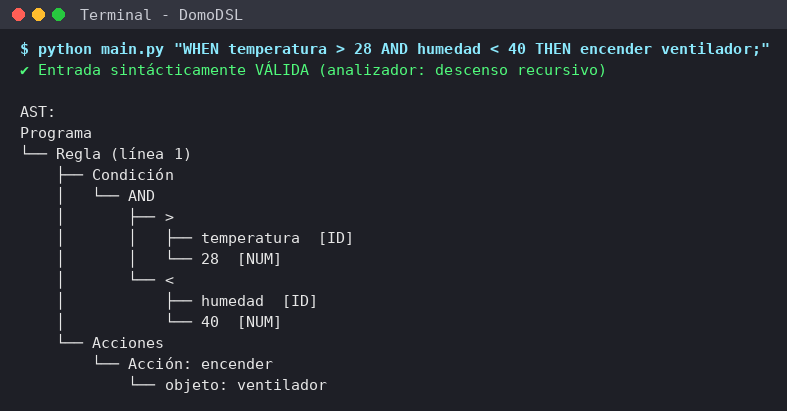
\includegraphics[width=0.78\textwidth]{../docs/img/cap_valida.png}
\caption{Entrada válida: se informa el resultado y se imprime el AST.}
\end{figure}
\begin{figure}[H]\centering
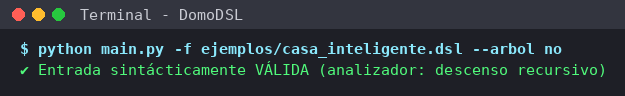
\includegraphics[width=0.95\textwidth]{../docs/img/cap_archivo.png}
\caption{Análisis de un archivo con cuatro reglas (\texttt{ejemplos/casa\_inteligente.dsl}).}
\end{figure}
\begin{figure}[H]\centering
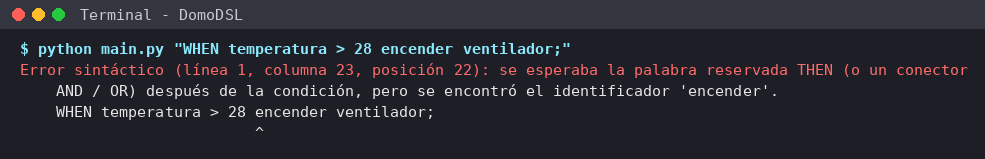
\includegraphics[width=0.95\textwidth]{../docs/img/cap_error_then.png}
\caption{Error sintáctico: falta \texttt{THEN}.}
\end{figure}
\begin{figure}[H]\centering
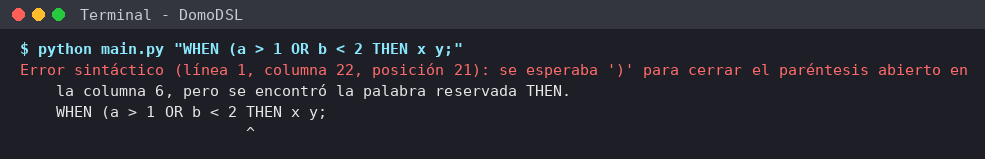
\includegraphics[width=0.95\textwidth]{../docs/img/cap_error_parentesis.png}
\caption{Error sintáctico: paréntesis sin cerrar.}
\end{figure}
\begin{figure}[H]\centering
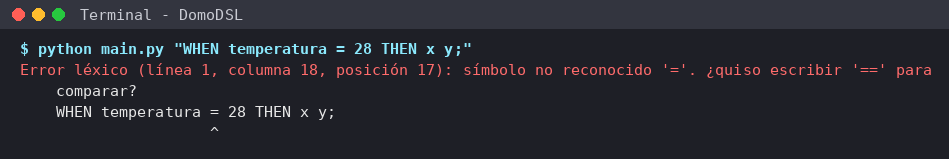
\includegraphics[width=0.95\textwidth]{../docs/img/cap_error_lexico.png}
\caption{Error léxico: \texttt{=} en lugar de \texttt{==}.}
\end{figure}
\begin{figure}[H]\centering
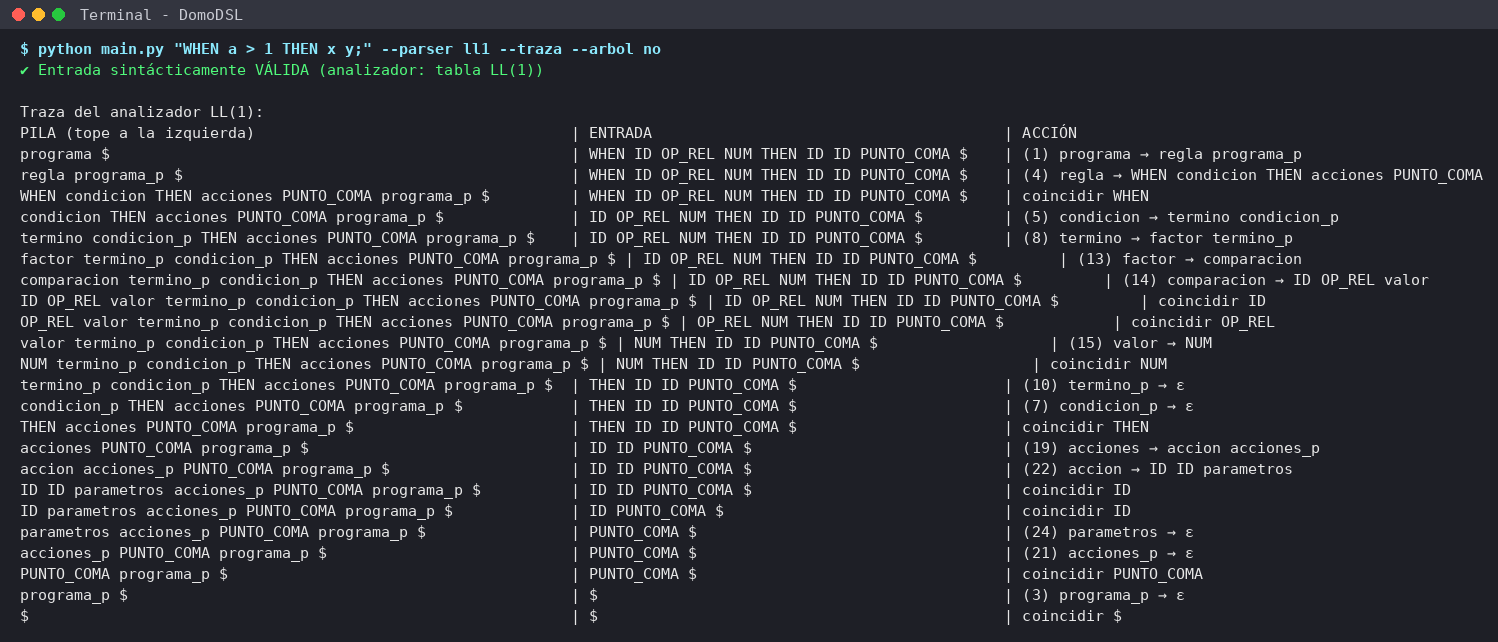
\includegraphics[width=\textwidth]{../docs/img/cap_traza_ll1.png}
\caption{Traza del analizador LL(1) (\texttt{--traza}): pila, entrada restante y producción aplicada.}
\end{figure}
\begin{figure}[H]\centering
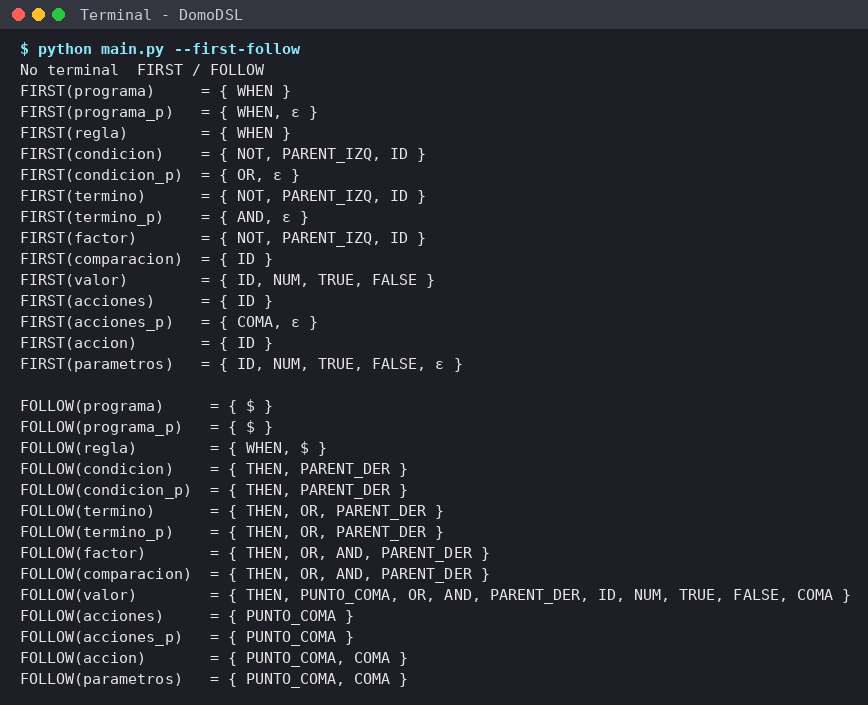
\includegraphics[width=0.85\textwidth]{../docs/img/cap_first_follow.png}
\caption{FIRST y FOLLOW calculados por el programa (\texttt{--first-follow}).}
\end{figure}
\begin{figure}[H]\centering
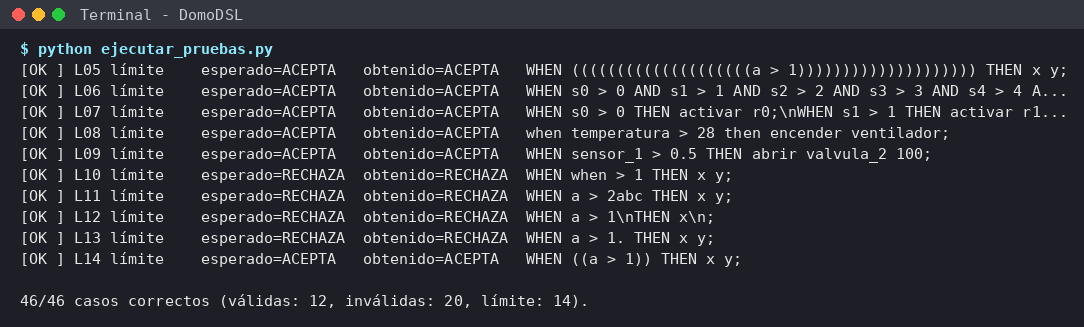
\includegraphics[width=0.95\textwidth]{../docs/img/cap_pruebas.png}
\caption{Resultado de \texttt{ejecutar\_pruebas.py}.}
\end{figure}
\begin{figure}[H]\centering
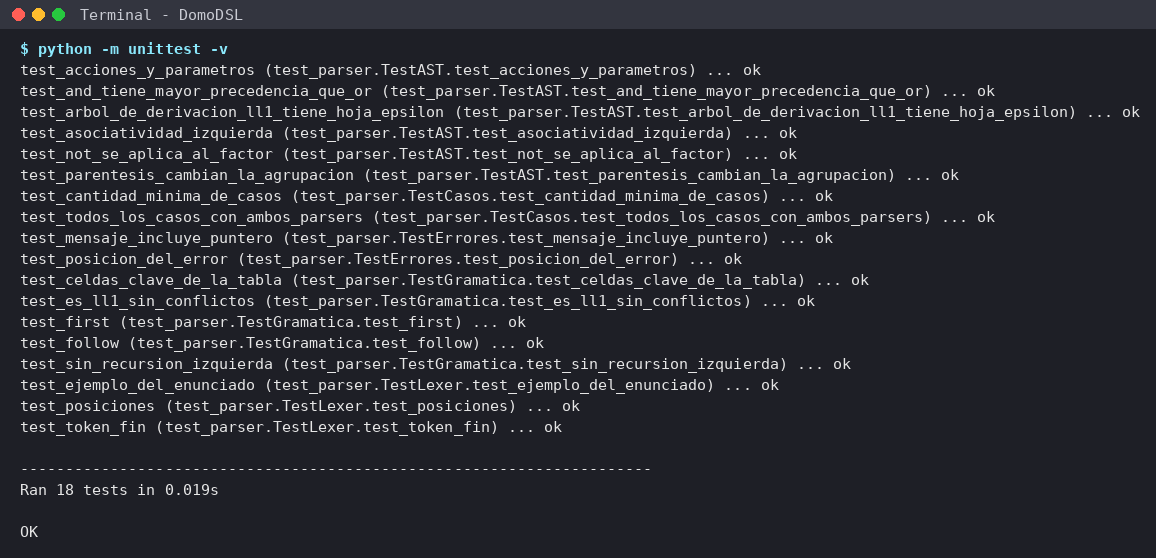
\includegraphics[width=0.95\textwidth]{../docs/img/cap_unittest.png}
\caption{Resultado de las pruebas unitarias.}
\end{figure}

\clearpage
\subsection*{Anexo C. Código fuente de los módulos principales}
\lstinputlisting[caption={lexer.py --- analizador léxico}]{../lexer.py}
\lstinputlisting[caption={gramatica.py --- GLC, FIRST, FOLLOW y tabla LL(1)}]{../gramatica.py}
\lstinputlisting[caption={parser\_rd.py --- parser por descenso recursivo}]{../parser_rd.py}
\lstinputlisting[caption={parser\_ll1.py --- parser dirigido por tabla LL(1)}]{../parser_ll1.py}

\fi
   % secciones 10, 11 y 12 (parte 2)
\end{document}
